\section{生命周期}
在之前的所有权一节,有这么一个函数示例:
\begin{code-block}{rust}
fn first_word(s: &str) -> &str {
    return &s[..];
}

fn copy_ref(s: &str) -> &str {
    // 也可以是&s,为啥?
    return s;
}
\end{code-block}
上述的函数都运行正常。对函数进行改造,改造成下列的样式:
\begin{code-block}{rust}
fn longest(x: &str, y: &str) -> &str {
    if x.len() > y.len() {
        x
    } else {
        y
    }
}
\end{code-block}
即,返回2个字符串当中最长的。如果对这样的代码进行编译,则会出现错误:
\begin{figure}[H]
  \centering
  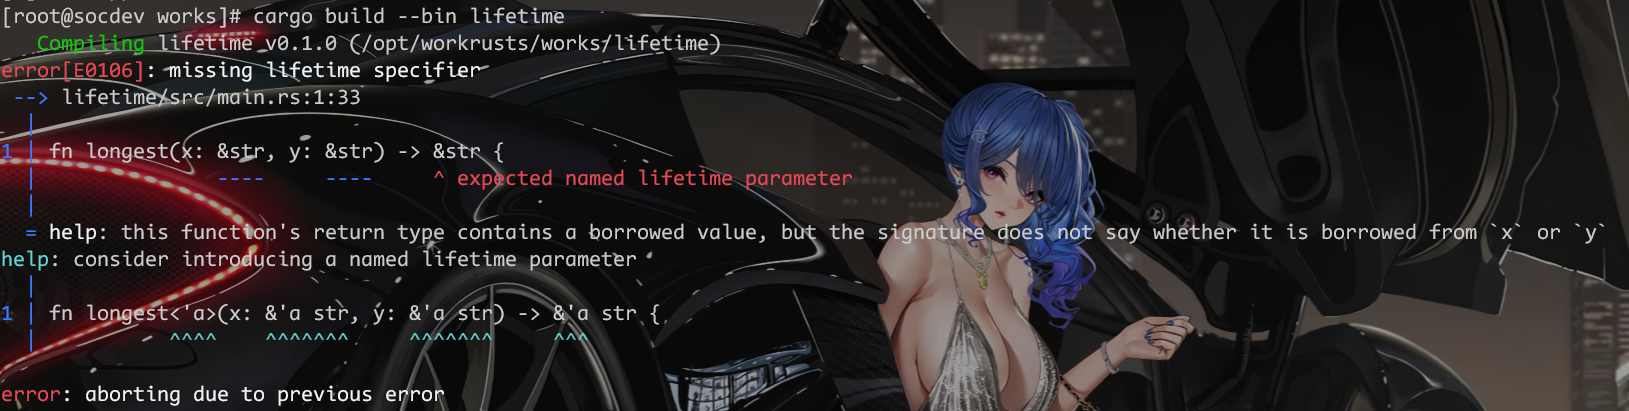
\includegraphics[width=\linewidth]{rust_strref_err.png}
  \caption{试图返回多个引用当中的某一个}
  \label{fig:rust_strref_err}
\end{figure}
错误表示,函数应该返回一个有生命周期的命名变量。错误的原因是,Rust编译器无法知道
函数返回的到底是x还是y的引用,无法确定对应的变量的生命周期。

Rust当中,针对引用和借用,有一个特殊的机制:借用检查器,其作用比较作用域来确保所
有的借用都是有效的。
\begin{code-block}{rust}
{
    let r;                      // ---------+-- 'a
    {                            //          |
        let x = 5;             // -+-- 'b  |
        r = &x;                 //  |       |
    }                            // -+       |
    println!("r: {}", r); // ---------+
}
\end{code-block}

其中'a表示变量r原本的作用域(生命周期),'b则表示变量x的有效作用域。进入'b作用域
之后,r变量引用了一个作用域为'b的变量x,当退出'b之后,x失去作用,导致作为x的引用
的r也失去作用,被回收,因此,上述代码无法进行编译:'b的作用范围比'a要小。

为了解决这类的问题,Rust引入了生命周期的操作。生命周期的定义通常使用'+名称的方式
进行定义,表示一个变量或者函数的有效范围,如下:
\begin{code-block}{rust}
&i32        // 引用
&'a i32     // 带有显式生命周期的引用
&'a mut i32 // 带有显式生命周期的可变引用
\end{code-block}
生命周期不仅可以用于变量,同样可以作用与函数和方法上:
\begin{code-block}{rust}
fn main() {
    let string1 = String::from("abcd");
    let string2 = "xyz";

    let res = longest(&string1, string2);
    println!("The result is {}", res);
    println!("The result is {}", res);
}

fn longest<'a>(x: &'a str, y: &'a str) -> &'a str {
    if x.len() > y.len() {
        x
    } else {
        y
    }
}
\end{code-block}
上述代码表示,参数列表当中的所有引用都必须拥有相同的生命周期'a,通过生命周期的限定,
上述代码可以正常编译,并且正常执行。需要注意,如果在参数上使用生命周期,则函数/方法
的前面,则必须加上生命周期,否则会提示参数列表当中的生命周期没有定义。

生命周期同样可以应用于结构体字段定义当中,如下:
\begin{code-block}{rust}
struct ImportantExcerpt<'a> {
    part: &'a str,
}
\end{code-block}

上述结构体的初始化,则可以直接使用字符串的引用进行实现:
\begin{code-block}{rust}
let i = ImportantExcerpt { part: "zhangjl" };
println!("{}", i.part);
\end{code-block}

对于带有生命周期的结构体,在使用的时候,尤其是函数定义和方法定义时,有一些必须
注意的细节:
\begin{outline}[enumerate]
\1 传入外部引用数据模式

使用这种模式,通常情况下,不需要对函数添加生命周期,和普通函数相同。不过,也可以
使用添加生命周期的完整形式:
\begin{code-block}{rust}
fn init_struct(source: &str) -> ImportantExcerpt {
    return ImportantExcerpt { part: source };
}

// 使用生命周期的完整形式,实际上是上述函数的完整签名形式
// fn init_struct<'a>(source: &'a str) -> ImportantExcerpt<'a> {
//     return ImportantExcerpt { part: source };
// }

...

// 调用函数
let b = init_struct("luoyan");
\end{code-block}
由于上述代码当中,结构体的变量的有效生命周期和外部引用的相同,因此,可以简化生命
周期的使用。

\1 使用函数局部变量

在这种方式下,由于局部引用变量的作用域有限,返回函数之后就不存在了,因此,必须使用
显式的生命周期,而显式的生命周期使用同样有2种形式:
\begin{code-block}{rust}
fn init_struct<'a>() -> ImportantExcerpt<'a> {
    return ImportantExcerpt { part: "luoyan"};
}

// 使用静态生命周期,'static表示静态生命周期,为固定关键字
// fn init_struct() -> ImportantExcerpt<'static> {
//     return ImportantExcerpt { part: "luoyan"};
// }
\end{code-block}

\1 实现Trait

包含有引用数据类型的结构体,也可以实现各种标准库的Trait。在实现Trait的时候,也
必须使用生命周期:
\begin{code-block}{rust}
// 可替换成下面的代码
// impl<'a> fmt::Display for ImportantExcerpt<'a> {
// static可以替换为_
impl fmt::Display for ImportantExcerpt<'static> {
    fn fmt(&self, f: &mut fmt::Formatter) -> fmt::Result {
        write!(f, "{}", self.part)
    }
}
\end{code-block}

\1 添加结构体方法

结构体存在引用数据类型,同样要求结构体的方法在实现时需要进行额外的处理,添加生命
周期的使用,同样的,结构体的方法可以使用命名生命周期,也可以使用固定生命周期:
\begin{code-block}{rust}
// 使用命名生命周期的结构体方法声明
impl<'a> ImportantExcerpt<'a> {
    fn show(&self) {
        println!("{}", self.part);
    }
    fn reset(&mut self, other: &'a str) {
        self.part = other;
    }
    fn get(&self) -> &str {
        return self.part;
    }
}

// 使用固定生命周期的结构体方法声明
impl ImportantExcerpt<'static> {
    fn show(&self) {
        println!("{}", self.part);
    }
    fn reset(&mut self, other: &'static str) {
        self.part = other;
    }
    fn get(&self) -> &str {
        return self.part;
    }
}
\end{code-block}

\end{outline}

在上述的代码当中,很多地方都使用了'static静态生命周期。这是一种特殊的生命周期,
能够存活于整个程序期间,所有的字符串字面值都拥有'static生命周期。但是,并不是
任何情况都建议使用static生命周期。

由于生命周期和泛型以及Trait都非常类似,不可避免的,有可能会遇到几者合用的的情况,
在使用的时候,需要将生命周期与泛型使用,分割开,并且,生命周期应当放在首位。
\begin{code-block}{rust}
fn longest_with_an_announcement<'a, T>(x: &'a str, y: &'a str, ann: T) -> &'a str
    where T: Display
{
    println!("Announcement! {}", ann);
    if x.len() > y.len() {
        x
    } else {
        y
    }
}
\end{code-block}

当存在多个生命周期需求的时候,为了表示生命周期长短,则需要使用冒号:
\begin{code-block}{rust}
fn test<'a, 'b>(arg: &'a T) -> &'b i32
// 表示a的生命周期必须比b要长
where 'a:'b
{
    &arg.member
}
\end{code-block}

\section{测试}
Rust的测试与其他语言相同,分为单元测试和集成测试。但不管是单元测试,还是集成测试,
在测试当中,都需要遵循相同的测试规则。在默认的lib类型的crate当中,默认情况下,自动
生成的lib.rs会生成如下的代码:
\begin{code-block}{rust}
#[cfg(test)]
mod tests {
    #[test]
    fn it_works() {
        assert_eq!(2 + 2, 4);
    }
}
\end{code-block}
其中,\#[cfg(test)]表示这是一个测试模块,而\#[test]则表示接下来的函数或者方法是测试
函数,it\_works表示测试的函数/方法名,可以变更为其他的名称。其中,assert!、assert\_eq!
和assert\_ne!这3个宏定义,用于检测运行结果、是否相等/是否不等,比如检测返回值当中
是否包含特定的字符串:
\begin{code-block}{rust}
pub fn greeting(name: &str) -> String {
    format!("Hello {}!", name)
}
#[cfg(test)]
mod tests {
    // 引用暴露的模块代码
    use super::*;
    #[test]
    fn greeting_contains_name() {
        let result = greeting("Carol");
        assert!(result.contains("Carol"));
    }
}
\end{code-block}

如果需要测试panic的代码,则可以使用should\_panic宏进行,该宏表示期望对应的函数在
运行的时候出现panic:
\begin{code-block}{rust}
pub struct Guess {
    value: i32,
}
impl Guess {
    pub fn new(value: i32) -> Guess {
        if value < 1 || value > 100 {
            panic!("Guess value must be between 1 and 100, got {}.", value);
        }
        Guess {
            value
        }
    }
}
#[cfg(test)]
mod tests {
    use super::*;
    #[test]
    #[should_panic]
    fn greater_than_100() {
        Guess::new(200);
    }
}
\end{code-block}
如果测试失败,想在测试结果当中,提示出具体的测试错误信息,则可以添加should\_panic
属性中的expected参数:
\begin{code-block}{rust}
#[cfg(test)]
mod tests {
    use super::*;
    #[test]
    #[should_panic(expected = "Guess value must be between 1 and 100")]
    fn greater_than_100() {
        Guess::new(200);
    }
}
\end{code-block}

运行测试用例时,只需要简单的输入如下的指令即可:
\begin{code-block}{bash}
// 默认并行的方式运行所有的测试用例
cargo test
// 串行的方式运行所有的测试用例
cargo test -- --test-threads=1
// 运行指定的测试用例,可匹配以add开头的所有测试用例
cargo test add
\end{code-block}

需要单独说明的是Rust的集成测试。集成测试通常针对lib型的crate。其测试过程大致如下:
\begin{outline}[enumerate]
\1 创建一个lib,并编写代码

\begin{code-block}{bash}
cargo new --lib shared
\end{code-block}

\1 在shared的src同级目录下,创建集成测试用例目录:
\begin{code-block}{bash}
# 文件夹名称固定为tests
mkdir tests
\end{code-block}

\1 在tests下创建集成测试用例
\begin{code-block}{bash}
echo > tests/units.rs<<EOF
// 导入的lib名称必须是当前crate的名称
use shared;
#[test]
fn it_adds_two() {
    assert_eq!(4, adder::add_two(2));
}
EOF
\end{code-block}
然后执行测试即可。
\end{outline}

\section{Rust的函数式编程}
Rust同样支持函数式编程。相比于其他语言,Rust的函数式编程性能和效率更高。Rust常见的
函数式编程模式包括闭包和迭代器2大类。

\subsection{闭包}
Rust的闭包和Python当中的非常类似,都可以直接读取外部的变量。其定义的形式基本如下:
\begin{code-block}{rust}
let expensive_closure = |num| {
    println!("calculating slowly...");
    num * 10
};
let res = expensive_closure(10);
\end{code-block}
其中两个||表示定义一个闭包,中间的num表示闭包的参数。如果闭包需要处理多个参数,则
应该改写为:
\begin{code-block}{rust}
let expensive_closure = |num1, num2| { num1 * num2 };
\end{code-block}

从实际的使用当中可以看到,Rust的闭包实际上就是一个匿名函数,在Rust当中,函数都有
参数类型/返回值的声明,但是,在上述的代码当中,却没有看到相关的定义和声明。这是
因为Rust的闭包通常很短,并只关联于小范围的上下文而非任意情境。在这些有限制的上下
文中,编译器有能力可靠的推断参数和返回值的类型,如同能够推断大部分变量的类型一样。
不过,不注明参数/返回类型,有可能出现一种迷惑性的使用:即无法传入正确的数据类型,
如下:
\begin{code-block}{rust}
let example_closure = |x| x;
let s = example_closure(String::from("hello"));
let n = example_closure(5);
\end{code-block}
按照上述代码的定义,example\_closure只是将输入参数原封不动的返回给调用者,第1次
调用时,编译器会将该闭包推断为输入/输出为字符串类型,然后这些类型信息会被锁定到
该闭包当中。后续再传入数值,由于闭包的类型已经锁定,要求传入字符串,但实际传入的
是数值,结果就会导致上述代码出现错误:
\begin{figure}[H]
  \centering
  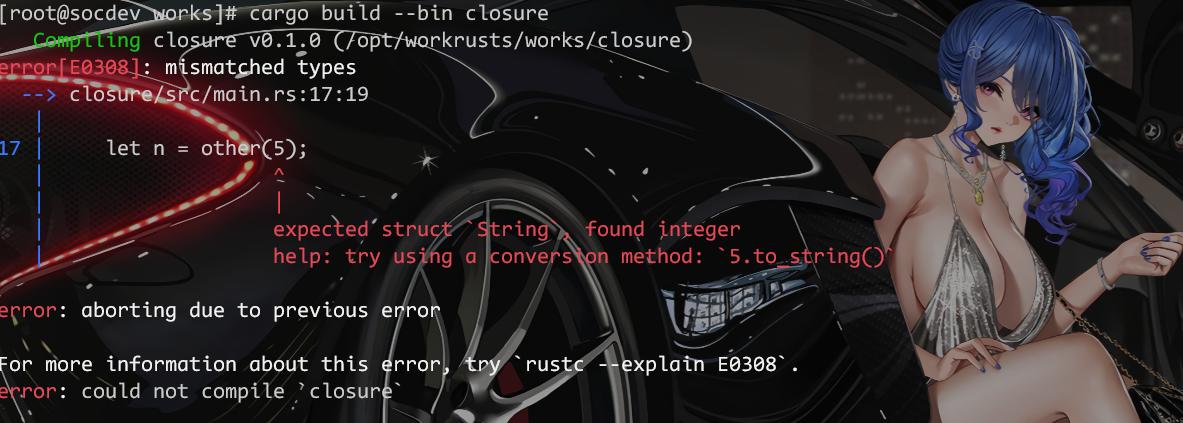
\includegraphics[width=\linewidth]{rust_closure_diffrent_type.png}
  \caption{试图处理不同数据类型的闭包}
  \label{fig:rust_closure_diffrent}
\end{figure}

闭包的完整定义(包括类型)则如下:
\begin{code-block}{rust}
let live_closure = |num: i32| -> (i32, i32) {
    println!("calculating slowly...");
    thread::sleep(Duration::from_secs(2));
    (num * 10, num * 20) // 或者修改为return语句 return (num*10, num*20);
};
// 如果不需要返回值,则闭包的写法需要注意一下:
let other = |x| { println!("{}", x); };
\end{code-block}

\subsection{特殊的闭包}
默认的情况下,包括Python和Golang,闭包都只是匿名函数。不过,在Rust当中,闭包可以
用在结构体当中,其主要用途就是memoization或lazy evaluation(惰性求值),即懒加载。
当结构体当中存放闭包时,则必须注明闭包的类型。而在结构体/枚举当中使用闭包,则需要
使用trait和泛型:Fn、FnMut和FnOnce。这3者的区别如下:
\begin{enumerate}
  \item FnOnce:闭包内对外部变量存在转移操作,导致外部变量不可用,所以只能call一次
  \item FnMut:闭包内对外部变量直接使用,并进行修改
  \item Fn:闭包内对外部变量直接使用,不进行修改
\end{enumerate}

使用这些trait的时候,则必须注明闭包的参数/返回值的类型。比如,闭包接收一个u32的
参数,返回一个u32,则对应的Fn trait bound则如下:
\begin{code-block}{rust}
Fn(u32) -> u32
\end{code-block}

一个包含闭包的结构体示例如下:
\begin{code-block}{rust}
struct Cacher<T>
where T: Fn(u32) -> u32,
{
    calculation: T,
    value: Option<u32>,
}
\end{code-block}
对该结构体的解读如下:结构体Cacher包含一个泛型calculation,而这个泛型则是一个使用
了Fn的闭包,这个闭包接收一个u32的参数,并最终返回一个u32。Value则是用于存放calculation
的计算结果,便于第二次调用时,直接返回而无需计算。根据上述需求,整个结构体的方法
实现如下:
\begin{code-block}{rust}
impl<T> Cacher<T>
where T: Fn(u32) -> u32,
{
    pub fn new(calculation: T) -> Cacher<T> {
        Cacher {
            calculation: calculation,
            value: None,
        }
    }
    pub fn value(&mut self, arg: u32) -> u32 {
        match self.value {
            Some(v) => v,
            None => {
                let v = (self.calculation)(arg);
                self.value = Some(v);
                v
            }
        }
    }
}
\end{code-block}
注意,在上述的结构体以及结构体方法当中,首次出现了trait bound和where的使用。需要
特别说明事实,trait bound几乎可以用于Rust的任何场景。New方法接收一个泛型作为初始化
参数,这个泛型就是一个Fn的闭包;而value方法则是根据根据当前结构体的数据,直接进行
数据的返回,或者计算,再返回。该结构体的使用方式如下:
\begin{code-block}{rust}
let mut cacher = Cacher::new(|x: u32| -> u32 { x * 10 });
let mut val = cacher.value(32);
println!("The val of cacher is {}", val);
val = cacher.value(45);
println!("The val of cacher second time is {}", val);
\end{code-block}
只是稍微可惜的是,这个表示缓存的结构体还存在bug,2次传入不同的数据,却得到了相同的
结果。问题在于字段value的定义。可以考虑使用Hashmap或者其他数据类型来替换value。一种
可能的解决方法如下:
\begin{code-block}{rust}
struct Cacher<T>
where T: Fn(u32) -> u32,
{
    calculation: T,
    value: BTreeMap<u32, Option<u32>>,
}

impl<T> Cacher<T>
where T: Fn(u32) -> u32,
{
    pub fn new(calculation: T) -> Cacher<T> {
        Cacher {
            calculation: calculation,
            value: BTreeMap::new(),
        }
    }
    pub fn value(&mut self, arg: u32) -> u32 {
        // 从现有的结果记录当中查询是否存在arg对应的计算结果
        match self.value.get(&arg) {
            // 找到则直接返回
            Some(Some(x)) => *x,
            // 没有找到,则计算一次,并放入当前的结果集合
            Some(None) | None => {
                let v = (self.calculation)(arg);
                self.value.insert(arg, Some(v));
                v
            }
        }
    }
}
\end{code-block}

闭包同样可以捕获运行环境的上下文,即在闭包内部直接使用外部的所有变量:
\begin{code-block}{rust}
fn main() {
    let x = 4;
    let equal_to_x = |z| z == x;
    let y = 4;
    assert!(equal_to_x(y));
}
\end{code-block}
X在闭包出现之前已经存在,定义闭包equal\_to\_x的时候,可以直接使用外部的x,而无需
重新声明。

\subsection{迭代器}
迭代器是Rust函数式编程的另外一个利器,负责遍历序列中的每一项和决定序列何时结束的
逻辑,我们在使用的时候,就无需判断开始条件和结束条件。在Rust当中,迭代器是惰性的,
只有使用到了,才会在内存当中进行展开。Rust的迭代器必须实现一个Iterator的triat,
这个trait的定义类似如下的结构:
\begin{code-block}{rust}
pub trait Iterator {
    type Item;
    fn next(&mut self) -> Option<Self::Item>;
}
\end{code-block}
其中的type Item和Self::Item定义了trait的关联数据类型,即该trait要求同时定义一个
Item类型,该类型被用作next方法的返回值类型。Next方法是Iterator被要求实现的唯一
方法,其一次返回一个项,最后返回一个None。

Rust的next方法得到的是迭代器的不可变引用,iter方法生成一个不可变引用的迭代器。
如果我们需要一个获取所有权并返回拥有所有权的迭代器,则可以调用into\_iter而不是iter。
类似的,如果我们希望迭代可变引用,则可以调用iter\_mut而不是iter;如果一旦调用了
into\_iter,则迭代完成之后,迭代器不再有效,比如下方代码:
\begin{code-block}{rust}
let v = vec![1, 2, 3];
let v3: Vec<_> = v.into_iter().map(|x| x * 12).collect();
println!("{:?}", v3);
println!("{:?}", v);
\end{code-block}
一旦进行编译,则会提示如下的错误:
\begin{figure}[H]
  \centering
  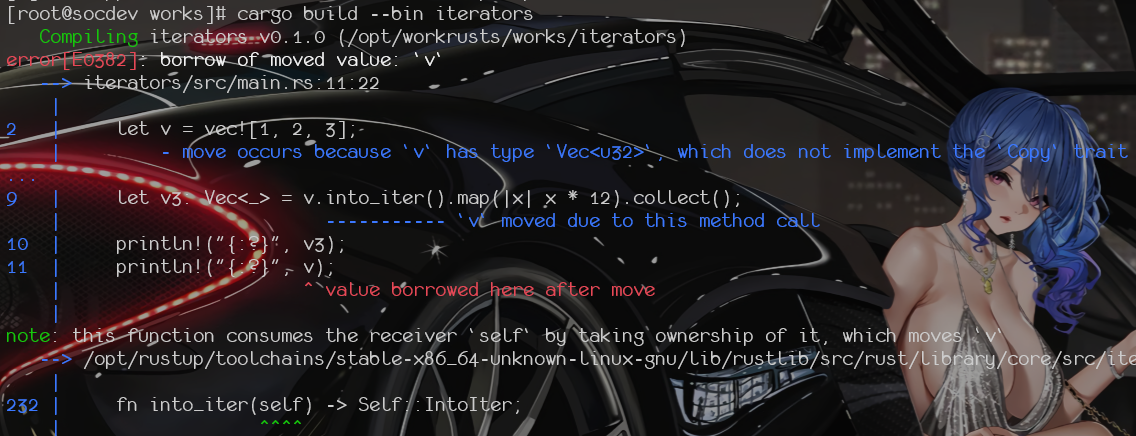
\includegraphics[width=\linewidth]{rust_iter_move.png}
  \caption{迭代器的所有权转移}
  \label{fig:rust_iter_move}
\end{figure}

实际上,上述的操作相当于对一个迭代器进行了消费。一般说来,调用next方法的方法被称为
消费适配器(consuming adaptors),因为调用他们会消耗迭代器。一个消费适配器的例子
是sum方法。这个方法获取迭代器的所有权并反复调用next来遍历迭代器,因而会消费迭代器。
当其遍历每一个项时,它将每一个项加总到一个总和并在迭代完成时返回总和。在这个过程
完成之后,原有的迭代器将无法再继续使用,因为其所有权已经进行了转移。
\begin{code-block}{rust}
let v = vec![1, 2, 3];
let v_item = v.iter();
let total1: u32 = v_item.sum();
// 迭代器v_item不再有效
println!("{:?}", v_item);
\end{code-block}

Iterator trait中定义了另一类方法,被称为迭代器适配器(iterator adaptors),允许
我们将当前迭代器变为不同类型的迭代器,并且可以链式调用多个迭代器适配器。不过因为
所有的迭代器都是惰性的,必须调用一个消费适配器方法以便获取迭代器适配器调用的结果。
比较常见的,就是使用map函数(迭代适配器,遍历迭代器的所有元素)来生成新的迭代器。
与之相对应的,collect方法则是消费迭代器并将结果收集到一个数据结构中。同样需要注意
的是,任何的迭代消费器,都不能进行类型的自动推导,需要手动的指定对应的数据类型。
比如,sum的结果通常是数值类型,而collect的结果则通常是vec类型。

迭代器和闭包通常结合使用,因为闭包可以捕获环境,比如常用的filter迭代器适配器:
\begin{code-block}{rust}
let v = vec![1, 2, 3];
// 使用的是iter,即引用数据类型,但是filter使用的本身是引用,因此,需要进行
// 2次的解引用操作
let res: Vec<_> = v.iter().filter(|s| *(*s) == 2).collect();
println!("{:?}", res);
// 原始的v仍然可用,没有发生所有权转移
println!("{:?}", v);
// 发生了所有权转移,变量v在后续的操作当中,无法被继续使用
let res1: Vec<_> = v.into_iter().filter(|s| *s == 2).collect();
println!("{:?}", res1);
\end{code-block}

Filter和迭代器使用的时候,需要特别注意所有权以及引用数据类型,特别是复合数据类型。
不同的操作会导致复合数据类型的所有权的变更。
\begin{code-block}{rust}
struct Shoe {
    size: u32,
    style: String,
}
fn main() {
    let shoes = vec![
        Shoe {
            size: 10,
            style: String::from("sneaker"),
        },
        Shoe {
            size: 13,
            style: String::from("sandal"),
        },
        Shoe {
            size: 10,
            style: String::from("boot"),
        },
    ];
    // 正确,返回的结果r实际上是shoes的部分数据的引用
    let r: Vec<_> = shoes.iter().filter(|x| x.size == 10).collect();
    // 错误,无法编译,由于collect返回的是引用,无法直接转换成引用原本的数据类型
    let r1: Vec<Shoes> = shoes.iter().filter(|x| x.size == 10).collect();
    // 正确,使用into_iter获取了相关的所有权,不再是引用,而是原始数据类型
    // 在此之后,shoes变量无法再使用,所有权已经发生了变更
    let r2: Vec<Shoes> = shoes.into_iter().filter(|x| x.size == 10).collect();
    // 错误,shoes的所有权已经发生了变更,此处已经无效
    shoes_in_my_size(shoes, 10);
}
// 调用者发生了所有权转移,调用该函数之后,参数shoes无法再被使用
fn shoes_in_my_size(shoes: Vec<Shoe>, shoe_size: u32) -> Vec<Shoe> {
    shoes.into_iter().filter(|s| s.size == shoe_size).collect()
}
\end{code-block}

\subsection{自定义迭代器}
可以通过在vector上调用iter、into\_iter或iter\_mut来创建一个迭代器,也可以用标准库
中其他的集合类型创建迭代器,比如哈希map。另外,可以实现Iterator trait来创建任何
我们希望的迭代器,如下:
\begin{code-block}{rust}
impl Counter {
    fn new(max: u32) -> Counter {
        return Counter {
            current: 0,
            max: max,
        };
    }
}

impl Iterator for Counter {
    type Item = u32;
    fn next(&mut self) -> Option<Self::Item> {
        self.current += 1;

        if self.current <= self.max {
            Some(self.current)
        } else {
            None
        }
    }
}
\end{code-block}
然后,即可像普通的集合数据类型Vec一样,使用for和next进行操作:
\begin{code-block}{rust}
let c = Counter::new(10);

// 忽略开头的n个数据
// for item in c.skip(1) {
// 像迭代器一样的使用类型
for item in c {
   println!("{}", item);
}

// 需要注意,c的所有权已经被转移,在此之后,无法再使用变量c

let c1 = Counter::new(10);
let c2 = Counter::new(20);

let sum: u32 = c1
    .zip(c2.skip(10))
    .map(|(a, b)| a * b)
    .filter(|x| x % 3 == 0)
    .sum();
println!("{}", sum);
\end{code-block}
上述的自定义迭代器并不完整,比如,默认情况下转移了变量的所有权,无法使用变量的引用
进行迭代等等。这些问题可以在后续进行进一步的改进。

\section{智能指针}
Rust当中同样存在指针,最常用的指针就包括引用数据类型。除了引用数据之外,引用类型
没有其他任何特殊的操作,也不存在其他额外的开销。除此之外,Rust还拥有智能指针,
这是一种数据结构,其表现类似于真正的指针,但是,拥有额外的元数据和功能。普通的引用
只是借用数据,而智能指针则是拥有指向的数据。

常见的智能指针包括String以及Vec<T>,通常使用结构体实现。和普通结构体明显区别的是,
智能指针实现了Deref和Drop这2个trait。Deref trait允许智能指针结构体实例表现的像引
用一样,这样就可以编写既用于引用、又用于智能指针的代码;Drop trait允许我们自定义
当智能指针离开作用域时运行的代码。在标准库当中最常用的智能指针主要包含下列3种:
\begin{enumerate}
  \item Box<T>:用于在堆上分配值
  \item Rc<T>:引用计数类型,其数据可以有多个所有者
  \item Ref<T> 和 RefMut<T>:通过RefCell<T>访问,RefCell<T>是一个在运行时而不是在编译时执行借用规则的类型
\end{enumerate}

\subsection{使用Box指向内存堆上的数据}
最简单直接的智能指针是box,其类型是 Box<T>。Box允许你将一个值放在堆上而不是栈上,
留在栈上的则是指向堆数据的指针。相比于普通的变量,Box的数据存放在内存堆上,但是
没有任何的性能损失,通常用于下列的场景当中:
\begin{itemize}
\item 当有一个在编译时未知大小的类型,而又想要在需要确切大小的上下文中使用这个类型值的时候
\item 当有大量数据并希望在确保数据不被拷贝的情况下转移所有权的时候
\item 当希望拥有一个值并只关心它的类型是否实现了特定trait而不是其具体类型的时候
\end{itemize}

第一种情况通常用于递归数据类型;第二种情况,转移大量数据的所有权会消耗大量的时间,
通过box将数据放在内存堆上,只有少量的指针数据在栈上被拷贝,减小了时间消耗;第三种
情况则通常称之为trait对象。

使用Box分配和使用堆上的数据示例如下:
\begin{code-block}{rust}
let v = Box::new(5);
let s = 10;

// Box类型无法直接和其他数据类型进行计算,必须进行转换
// 在本例当中,v的数据类型为Box<{integer}>
let b = v.as_ref() + s;
// 或者修改为如下的方式
// let b = *v + s;

println!("{}", b);
println!("{}", v);
\end{code-block}

Rust编译器要求在编译期间就能够确定对应的类型所占用的存储空间,但是,Rust当中也
存在无法在编译期间明确大小的数据类型,即递归数据类型。这种特殊类型的值,可以是
相同类型的另一个值,并且,这种嵌套关系可以无限进行下去,因此,Rust是不知道递归
数据类型的存储空间的。但是,可以通过在递归类型当中插入Box,以此为基准进行递归
数据类型的创建。

递归数据类型是一种特殊的数据类型,来源于Lisp,常见的开发语言当中没有与之相对的,
一个简单的递归数据类型的定义如下:
\begin{code-block}{rust}
enum List {
    Cons(i32, List),
    Nil,
}
\end{code-block}
Cons由2部分组成:自己包含的数据i32和另外一个List对象,其最后一项值包含一个叫做Nil
的值且没有下一项,代表递归的终止条件就是Nil。可以明显的看到,该数据类型理论上可
以无限的递归循环下去,我们无法在编译阶段就明确其存储空间占据的大小,因此上述代码
目前还无法编译通过。为了使得上述代码成功编译,可以利用Box特性:
\begin{code-block}{rust}
#[derive(Debug)]
enum List {
    Cons(i32, Box<List>),
    Nil,
}

use crate::List::{Cons, Nil};
fn main() {
    let list = Cons(1, Box::new(Cons(2, Box::new(Cons(3, Box::new(Nil))))));
    println!("{:?}", list);
}
\end{code-block}

通过这样的改变,Cons的大小就确定了:需要存放一个i32大小的值,以及一个Box指针大小
的数据(usize),从内存结构上看,其分布大致如下:
\begin{figure}[H]
  \centering
  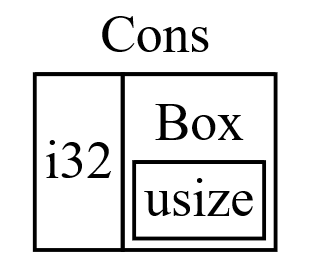
\includegraphics[scale=0.4]{rust_box.png}
  \caption{递归数据类型的内存示意}
  \label{fig:rust_box}
\end{figure}

\subsection{Deref Trait:将智能指针当作常规引用}
Deref Trait允许重载解引用操作符(*),将智能指针当作常规引用。在此之前,先看看
引用和原始数据之间的联系:
\begin{code-block}{rust}
let x = 5;
let y = &x;
// 正确,引用被转换成原始数据类型
let r = y + 9;
println!("{}, {}", y, r );
// 提示错误,代码无法进行编译和运行
println!("{}", y == 5);
// 提示错误,代码无法进行编译和运行
if y > 2 {
}
// 提示错误,代码无法进行编译和运行
assert_eq!(5, y);
// 正确,通过解引用,将引用变更为对应的类型
assert_eq!(5, y);
let mut yy = &x;
// 错误,无法编译
yy = yy + 10;
\end{code-block}
上述代码看起来是没有错误的,但是在编译的时候,会提示一个错误信息:
\begin{figure}[H]
  \centering
  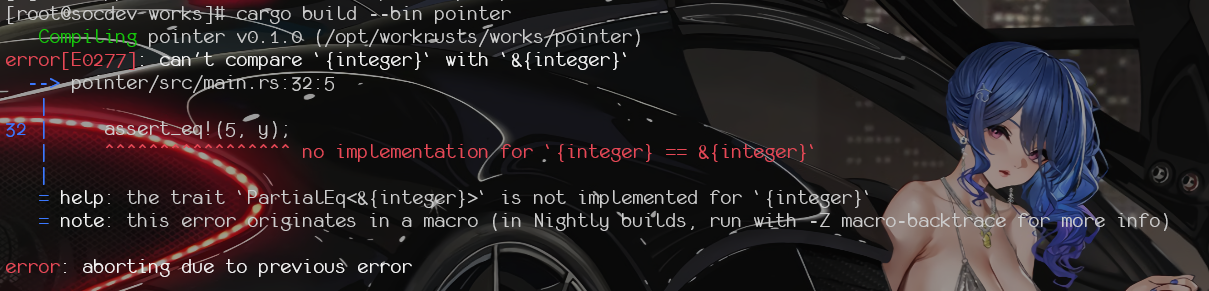
\includegraphics[width=\linewidth]{rust_pointer_error.png}
  \caption{尝试直接进行引用类型和其他类型的比较}
  \label{fig:rust_pointer_error}
\end{figure}
其根本原因在于,y虽然在使用上大多数情况和x没有什么区别,但是,实质上,y是一个引用
数据类型(指针),数值和x是具体的数值类型,引用和数值类型之间无法进行相互的比较。
如果需要进行对比,则需要对y进行解引用操作,或者直接使用原始的x。同样的,引用数据
类型和数值类型进行计算,得到的结果是数值类型,而并非引用数据类型。如果使用Box来替换
引用数据类型,其结果相同:
\begin{code-block}{rust}
let x = 5;
let y = Box::new(x);
// 提示错误,同样是由于数据类型不匹配
assert_eq!(5, y);
// 正确,通过解引用,将引用变更为对应的类型
assert_eq!(5, *y);
\end{code-block}

同样的,可以用Deref Trait实现自定义的智能指针。从本质上讲,Box<T>实际上是一个被
定义为包含一个元素的元组结构体(元组当中只包含一个元素),可以根据这个思路自定义
类似Box的智能指针:
\begin{code-block}{rust}
struct Pointer<T>(T);
impl<T> Pointer<T> {
    fn new(x: T) -> Pointer<T> {
        Pointer(x)
    }
}
\end{code-block}
上述代码使用泛型T作为元组的参数,使得该结构体可以嵌入/使用任何数据类型。接着实现
该结构的Deref Trait:
\begin{code-block}{rust}
impl<T> Deref for Pointer<T> {
    type Target = T; // 定义关联类型
    fn deref(&self) -> &T {
        &self.0
    }
}
\end{code-block}
也就是说,针对智能指针Pointer,已经可以实现对泛型数据的封装,并且可以正常的进行
解引用操作:
\begin{code-block}{rust}
// 代码可以正常的运行
let p = Pointer::new(5);
assert_eq!(5, *p);
let s = Pointer::new("lucifer");
assert_eq!("lucifer", *s);
\end{code-block}

在Rust当中,实现了Deref Trait的数据类型,在使用时,会将其引用转换为原始数据类型,
这种转换通常称之为解引用强制多态。当这种特定类型的引用作为实参传递给和形参类型
不同的函数或方法时,解引用强制多态将自动发生:
\begin{code-block}{rust}
fn hello(name: &str) {
    println!("Hello, {}!", name);
}
fn main() {
    let m = Pointer::new(String::from("Rust"));
    hello(&m);
}
\end{code-block}
上述代码当中,使用\&m调用hello函数,其为Pointer<String>值的引用,因为在Pointer<T>
上实现了Deref trait,Rust可以通过deref调用将Pointer<String>变为\&String,同时标准
库中提供了String上的Deref实现,其会返回字符串slice,Rust再次调用deref将\&String
变为\&str,这就符合hello 函数的定义了。

如果没有解引用强制多态的特性,则函数的调用则必须变更为如下的样式:
\begin{code-block}{rust}
hello(&(*m)[..]);
\end{code-block}
即(*m)将Pointer<String>解引用为String。接着\&和[..]获取了整个String的字符串slice
来匹配hello的签名,这无疑是一种低效的使用方式。

Deref重载的是不可变引用的*运算符,DerefMut则用于重载可变引用的*运算符。当发现如下
的几种情况时,Rust会进行解引用的强制多态:
\begin{itemize}
  \item 当T: Deref<Target=U> 时从\&T到\&U
  \item 当T: DerefMut<Target=U> 时从\&mut T到\&mut U
  \item 当T: Deref<Target=U> 时从\&mut T到\&U
\end{itemize}
第一种情况表明如果有一个\&T,而T实现了返回U类型的Deref,则可以直接得到\&U;第二种
情况表明对于可变引用也有着相同的行为;第3种情况,将可变引用强转为不可变引用,但
反过来是不行的,即不可变引用永远也不能强转为可变引用。

\subsection{使用Drop trait清理}
对于智能指针模式来说第二个重要的trait是Drop,其允许我们在值要离开作用域时执行一
些代码。默认可以为任何类型提供Drop trait的实现,同时所指定的代码被用于释放类似
于文件或网络连接的资源。

在其他一些语言中,我们不得不记住在每次使用完智能指针实例后调用清理内存或资源的代码。
如果忘记的话,运行代码的系统可能会因为负荷过重而崩溃。在Rust中,可以指定每当值离
开作用域时被执行的代码,编译器会自动插入这些代码,不需要在程序中到处编写在实例结
束时清理这些变量的代码,而且还不会出现内存泄漏。

Drop trait比较类似于C++的析构函数,用于指定对应的对象在离开作用域时需要进行的清理
代码,要求实现一个drop函数。简单的示例如下:
\begin{code-block}{rust}
struct SmartPointer {
    data: String,
}
impl Drop for SmartPointer {
    fn drop(&mut self) {
        println!("Drop the smart pointer {}", self.data);
    }
}
fn main() {
    let p = SmartPointer::new("zhangjl");
}
\end{code-block}
虽然在main函数当中,没有执行任何的输出操作,但是当代码结束运行时,还是会打印出
drop函数的执行结果,就如同析构函数一般。但和析构函数不同的是,析构函数可以通过
del操作调用,而Rust的drop函数是无法调用或者禁用的。如果需要提前释放变量,则需要
使用std::mem::drop进行替换:
\begin{code-block}{rust}
fn main() {
    let p = SmartPointer::new("zhangjl");
    drop(p);
    println!("Hello World");
}
\end{code-block}

\subsection{引用计数智能指针}
在Rust当中,大部分情况下,变量的所有权是明确且单一的。但是,有的场景下,要求单个
值有多个所有者。例如,在图数据结构中,多个边可能指向相同的节点,而这个节点从概念
上讲为所有指向它的边所拥有,节点直到没有任何边指向它之前都不应该被清理。为了解决
类似的问题,Rust使用Rc<T>进行引用计数的表达。引用计数意味着记录一个值引用的数量
来知晓这个值是否仍在被使用,如果某个值有零个引用,就代表没有任何有效引用并可以
被清理,反之则必须保留。特别注意的是,Rc<T>只能用于单线程/单进程环境。

简单的Rc使用示例如下:
\begin{code-block}{rust}
use std::rc::Rc;
struct User {
    name: String,
}
fn main() {
    let u = User {
        name: "zhangjl".to_string(),
    };
    let u_ref = Rc::new(u);
    println!("{}", u_ref.as_ref().name);
    let u_ref2 = Rc::clone(&u_ref);
}
\end{code-block}
Rc::clone的实现并不像类型的clone方法实现的是深拷贝一样,该函数只会增加对象的引用
计数,因此类型的clone方法可能会消耗大量的时间,而Rc::clone并不会耗费额外的时间。
Rc允许一个值有多个所有者,不过,它只允许以只读的方式进行共享数据,如果需要对数据
进行更改,则必须利用内部可变性模式以及RefCell类型,以此解决Rc的只读限制。

内部可变性是一种Rust的设计模式,这种模式允许即使在有不可变引用的时候,也可以进行
数据的改变,其重点是在数据结构当中使用unsafe来模糊Rust通常的可变性和借用规则。Unsafe
代码通常被封装进入安全的代码(API)当中,但是,外部类型仍然是不可变的。在不使用
unsafe代码的前提下,通常则是使用RefCell来进行数据的改变。

与Rc拥有多个所有者不同,RefCell代表的是数据的唯一所有权。在Rust当中,所有权和借用
规则是非常重要的:
\begin{enumerate}
  \item 在任意时刻,同一个变量只能拥有一个可变引用,或者任意数量的不可变引用
  \item 引用总是必须有效的
\end{enumerate}
如下代码:
\begin{code-block}{rust}
fn main() {
    let mut a = 24;
    add(&mut a);
    println!("{}", a);
    let mut b = &mut a;
    // 错误
    println!("{}, {}", b, a);
}
fn add(b: &mut u32) {
    *b = *b + 10
}
\end{code-block}

对于引用和Box,借用规则的不可变性表现在编译时期;对于RefCell,借用规则的不可变性
则体现在运行时期,因此,一旦RefCell违反了借用规则,则运行时将出现panic。同样的,
RefCell也只能使用于单线程/单进程场景。因此,在实质上,不管是RefCell还是其他,都
还是必须要遵循借用规则的。借用规则存在一个推论:当有一个不可变变量时,不能通过
可变引用借用他,如下:
\begin{code-block}{rust}
let x = 5;
let y = &mut x;
\end{code-block}
上述代码就会出现错误。

然而,在特定情况下,令一个值在其方法内部能够修改自身,而在其他代码中仍视为不可变,
是很有用的。RefCell<T>是一个获得内部可变性的方法,他并没有完全绕开借用规则,编译
器中的借用检查器允许内部可变性并相应地在运行时检查借用规则。如果违反了这些规则,
会出现panic而不是编译错误。如下的特殊情况,模拟Mock对象进行测试:
\begin{code-block}{rust}
pub trait Messager {
    fn send(&self, msg: &str);
}
pub struct LimitTracker<'a, T: Messager> {
    messager: &'a T,
    value: usize,
    max: usize,
}
impl<'a, T> LimitTracker<'a, T>
where
    T: Messager,
{
    pub fn new(messeger: &T, max: usize) -> LimitTracker<T> {
        LimitTracker {
            messager: messeger,
            value: 0,
            max: max,
        }
    }
    pub fn set_value(&mut self, value: usize) {
        self.value = value;
        self.messager
            .send(&format!("The value of tracker is {}", self.value));
    }
}
\end{code-block}

然后实现一个Messager,用于测试消息的发送,其实现如下:
\begin{code-block}{rust}
struct MockMessager {
    sent_messages: Vec<String>,
}
impl MockMessager {
    fn new() -> MockMessager {
        MockMessager {
            sent_messages: Vec::new(),
        }
    }
}
impl Messager for MockMessager {
    fn send(&self, message: &str) {
        self.sent_messages.push(String::from(message));
    }
}
\end{code-block}

按照我们的设想,测试的main函数应当如下:
\begin{code-block}{rust}
fn main() {
    let mock_messenger = MockMessager::new();
    let mut limit_tracker = LimitTracker::new(&mock_messenger, 100);
    limit_tracker.set_value(80);
    assert_eq!(mock_messenger.sent_messages.len(), 1);
}
\end{code-block}

但是,上述代码在进行编译时,则会出现错误:
\begin{figure}[H]
  \centering
  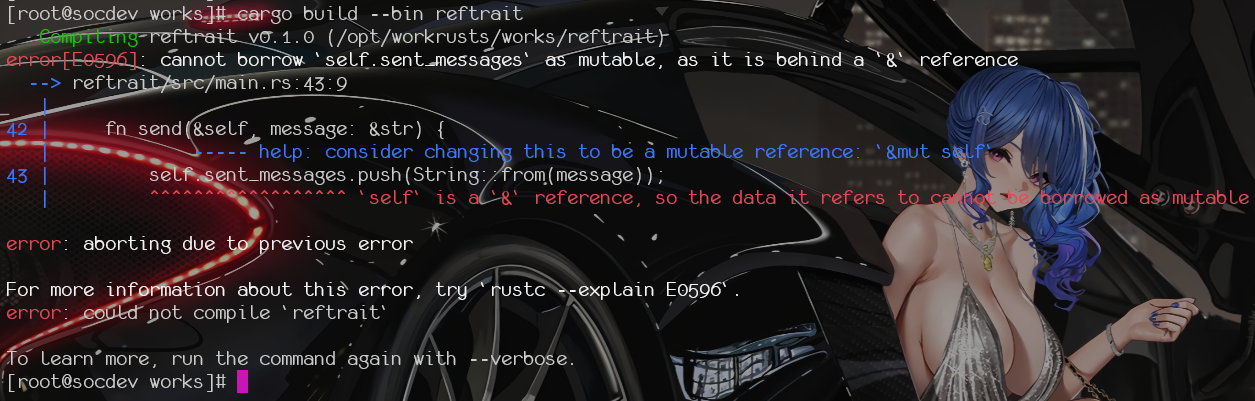
\includegraphics[width=\linewidth]{rust_ref_error.png}
  \caption{尝试修改不可变的引用}
  \label{fig:rust_ref_error}
\end{figure}

我们尝试去修改不可变的self引用的值,而这种情况,则正好可以利用RefCell进行实现,
其实现的代码如下:
\begin{code-block}{rust}
struct MockMessager {
    sent_messages: RefCell<Vec<String>>,
}
impl MockMessager {
    fn new() -> MockMessager {
        MockMessager {
            sent_messages: RefCell::new(Vec::new()),
        }
    }
}
impl Messager for MockMessager {
    fn send(&self, message: &str) {
        self.sent_messages.borrow_mut().push(String::from(message));
    }
}
fn main() {
    let mock_messenger = MockMessager::new();
    let mut limit_tracker = LimitTracker::new(&mock_messenger, 100);
    limit_tracker.set_value(80);
    assert_eq!(mock_messenger.sent_messages.borrow().len(), 1);
}
\end{code-block}
对于send方法的实现,第一个参数仍为self的不可变借用,这是符合方法定义的,调用
self.sent\_messages中RefCell的borrow\_mut方法来获取RefCell中值的可变引用,随之
就可以进行self当中的变量的修改了。

当创建不可变和可变引用时,我们分别使用\&和\&mut语法;对于RefCell<T>来说,则是
borrow和borrow\_mut 方法,这是属于RefCell<T>安全API的一部分。Borrow方法返回
Ref<T>类型的智能指针,borrow\_mut方法返回RefMut类型的智能指针。这两个类型都实现
了Deref,所以可以当作常规引用对待。但是,RefCell同样遵循借用规则,在任何时候只
允许有多个不可变借用或一个可变借用。

在实际使用当中RefCell常常和Rc结合使用:如果有一个储存了RefCell<T>的 Rc<T> 的话,
就可以得到有多个所有者并且可以修改的值了,比如下列的示例:
\begin{code-block}{rust}
use std::cell::RefCell;
use std::rc::Rc;
#[derive(Debug)]
enum List {
    Cons(Rc<RefCell<i32>>, Rc<List>),
    Nil,
}
use crate::List::{Cons, Nil};
fn main() {
    let value = Rc::new(RefCell::new(5));
    let a = Rc::new(Cons(Rc::clone(&value), Rc::new(Nil)));
    let b = Cons(Rc::new(RefCell::new(6)), Rc::clone(&a));
    let c = Cons(Rc::new(RefCell::new(10)), Rc::clone(&a));
    *value.borrow_mut() += 10;
    println!("a after = {:?}", a);
    println!("b after = {:?}", b);
    println!("c after = {:?}", c);
}
\end{code-block}
执行之后,其结果如下:
\begin{figure}[H]
  \centering
  
\includegraphics[width=\linewidth]{rust_ref_cell.png}
  \caption{Rc和RefCell修改多个引用的值}
  \label{fig:rust_ref_cell}
\end{figure}

\subsection{引用循环和内存泄漏}
Rust的内存安全性保证使其难以意外地制造永远也不会被清理的内存,即内存泄漏,但Rust
并不保证完全避免内存泄漏,但是,和其他语言不同的是,Rust的内存泄漏是安全的。在使用
智能指针时,特别是Rc和RefCell时,需要注意有可能出现的内存泄漏,如下代码所示:
\begin{code-block}{rust}
use crate::List::{Cons, Nil};
use std::cell::RefCell;
use std::rc::Rc;
#[derive(Debug)]
enum List {
    Cons(i32, RefCell<Rc<List>>),
    Nil,
}
impl List {
    fn tail(&self) -> Option<&RefCell<Rc<List>>> {
        match self {
            Cons(_, item) => Some(item),
            Nil => None,
        }
    }
}
\end{code-block}
现在Cons成员的第二个元素是RefCell<Rc<List>>,这意味着能够修改Cons成员所指向的List。
这里还增加了一个tail方法,允许其在有Cons成员的时候访问其第二项。在使用时候如下
进行操作:
\begin{code-block}{rust}
fn main() {
    let a = Rc::new(Cons(5, RefCell::new(Rc::new(Nil))));
    println!("a initial rc count = {}", Rc::strong_count(&a));
    println!("a next item = {:?}", a.tail());
    let b = Rc::new(Cons(10, RefCell::new(Rc::clone(&a))));
    println!("a rc count after b creation = {}", Rc::strong_count(&a));
    println!("b initial rc count = {}", Rc::strong_count(&b));
    println!("b next item = {:?}", b.tail());
    if let Some(link) = a.tail() {
        *link.borrow_mut() = Rc::clone(&b);
    }
    println!("b rc count after changing a = {}", Rc::strong_count(&b));
    println!("a rc count after changing a = {}", Rc::strong_count(&a));
    println!("a next item = {:?}", a.tail());
}
\end{code-block}
变量a中创建了一个Rc<List>实例来存放初值,变量b中创建了指向列表a的List的另一个Rc<List>
实例,也即是说,b是a的头部,a是b的尾部,a的尾部没有内容。但是,紧接着,将a的尾部
指向了b,就创建了一个循环,所以,在最后进行a的尾部输出的时候,就会导致整个程序栈溢出。

引用循环无法被Rust编译器所检查或者捕获到,由此带来的内存泄漏,Rust编译器同样无法
被检测到。解决这样的问题,一种是及时的使用测试工具以及单元测试进行排查,另外,则是
使用Weak替换Rc。

Rc::clone会增加Rc的强引用计数(strong\_count),只有当强引用计数归为0,对应的Rc才会
被清理。而Rc::downgrade则是创建Rc的弱引用,得到Weak类型的智能指针,但是,并不会增加
强引用计数,即不会改变strong\_count的数值,但是会增加弱引用计数(weak\_count)的
数值,不过,在使用当中,无需使得weak\_count为0,就可以回收Rc变量。总结的来说:
\begin{itemize}
  \item 强引用(strong\_count)表示共享Rc实例的所有权
  \item 弱引用(weak\_count)并没有所有权关系
  \item 任何弱引用的循环,都会在强引用计数为0时被打断
\end{itemize}

因为Weak<T>引用的值可能已经被丢弃了,为了使用Weak<T>所指向的值,我们必须确保其值
仍然有效,为此可以调用Weak<T>实例的upgrade方法,这会返回Option<Rc<T>>。如果Rc<T>
值还未被丢弃,则结果是Some;如果Rc<T>已被丢弃,则结果是 None,所以它不会返回非法
指针,进而导致程序崩溃。

关于弱引用,最简单的例子便是树形结构:父节点需要知道子节点,子节点也需要知道父节点,
但是,删除子节点,并不意味着父节点就失效了,父节点仍然是有效的;而删除父节点则不一样,
父节点被删除之后,其对应的子节点便已经无效了,对于这样的例子,其示例代码如下:
\begin{code-block}{rust}
#[derive(Debug)]
struct Node {
    value: i32,
    parent: RefCell<Weak<Node>>,
    children: RefCell<Vec<Rc<Node>>>,
}
\end{code-block}
即一个节点就能够引用其父节点,但不拥有其父节点。其使用示例如下:
\begin{code-block}{rust}
let leaf = Rc::new(Node {
    value: 3,
    parent: RefCell::new(Weak::new()),
    children: RefCell::new(vec![]),
});
println!("leaf parent = {:?}", leaf.parent.borrow().upgrade());

let branch = Rc::new(Node {
    value: 5,
    parent: RefCell::new(Weak::new()),
    children: RefCell::new(vec![Rc::clone(&leaf)]),
});

*leaf.parent.borrow_mut() = Rc::downgrade(&branch);
println!("leaf parent = {:?}", leaf.parent.borrow().upgrade());
\end{code-block}
\section{Match与模式匹配}
Match是Rust常用的语法糖,其用法不局限于之前所讲的范围。关于match的用法,还有很多,
并且,多数和模式匹配有关,接下来可以看一些常见的match和模式匹配的使用方式。
\begin{outline}[enumerate]
\1 多种匹配模式

在match表达式当中,可以用|匹配多个模式,表示或运算:
\begin{code-block}{rust}
let x = 1;
match x {
    1 | 2 => println!("one or two"),
    3 => println!("three"),
    _ => println!("anything"),
}
\end{code-block}

\1 使用..=匹配范围

..=语法允许匹配一个数值范围内的任意数据,常用于数值和字符:
\begin{code-block}{rust}
let x = 5;
match x {
    1..=5 => println!("one through five"),
    _ => println!("something else"),
}

let y = 'c';
match y {
    'a'..='j' => println!("early ASCII letter"),
    'k'..='z' => println!("late ASCII letter"),
    _ => println!("something else"),
}
\end{code-block}

\1 解构结构体

Let模式可以将结构体当中的字段/元素进行解构,单独或者批量赋予其他元素:
\begin{code-block}{rust}
struct Point {
    x: i32,
    y: i32,
}
fn main() {
    let p = Point { x: 0, y: 7 };
    // 将p的x字段的值赋予a,y字段的值赋予b,a和b是整数类型,不是引用
    let Point { x: a, y: b } = p;
    // let Point {x: ref a, y: ref b} = p; 和上面类似,但是a和b是整数类型的引用
    // let Point {x: a, y: _} = p; 表示只需要将x的值赋予a,但不需要对y进行解构
    assert_eq!(0, a);
    assert_eq!(7, b);
    // let Point {x, y} = p; 将p的x字段的值赋予变量x,y字段的值赋予变量y
}
\end{code-block}

\1 解构枚举类型

Match本身就是应枚举而生的,因此天然的可以使用它对枚举进行解构:
\begin{code-block}{rust}
enum Message {
    Quit,
    Move { x: i32, y: i32 },
    Write(String),
    ChangeColor(i32, i32, i32),
}
fn main() {
    let msg = Message::ChangeColor(0, 160, 255);
    match msg {
        Message::Quit => {
            println!("The Quit variant has no data to destructure.")
        }
        Message::Move { x, y } => {
            println!("Move in the x direction {} and in the y direction {}", x, y);
        }
        Message::Write(text) => println!("Text message: {}", text),
        Message::ChangeColor(r, g, b) => {
            println!("Change the color to red {}, green {}, and blue {}", r, g, b)
        }
    }
}
\end{code-block}

同样的,如果枚举当中嵌套了枚举,仍然可以使用match进行解构:
\begin{code-block}{rust}
enum Color {
    Rgb(i32, i32, i32),
    Hsv(i32, i32, i32),
}
enum Message {
    Quit,
    Move { x: i32, y: i32 },
    Write(String),
    ChangeColor(Color),
}
fn main() {
    let msg = Message::ChangeColor(Color::Hsv(0, 160, 255));
    match msg {
        Message::ChangeColor(Color::Rgb(r, g, b)) => {
            println!("Change the color to red {}, green {}, and blue {}", r, g, b)
        }
        Message::ChangeColor(Color::Hsv(h, s, v)) => {
            println!(
                "Change the color to hue {}, saturation {}, and value {}",
                h, s, v
            )
        }
        _ => (),
    }
}
\end{code-block}

\1 解构复合数据

用复杂的方式来混合、匹配和嵌套解构模式,解析出我们感兴趣的数据:
\begin{code-block}{rust}
let ((feet, inches), Point {x, y}) = ((3, 10), Point { x: 3, y: -10 });
\end{code-block}

\1 忽略不需要的元素

在Rust的当中,默认可以使用\_对不必要的变量进行忽略,通常用在match的最后分支,但是,
实际上也可以用去其他任意的模式,甚至是函数参数:
\begin{code-block}{rust}
// 需要传入2个参数,但是忽略第一个参数
fn foo(_: i32, y: i32) {
    println!("This code only uses the y parameter: {}", y);
}
fn main() {
    foo(3, 4);
}
\end{code-block}

除了使用\_进行忽略之外,还可以使用..语法糖进行忽略,但是针对结构体和元组存在区别:
结构体当中,忽略的是没有被列出的字段;而元组忽略的则是范围:
\begin{code-block}{rust}
struct Point {
    x: i32,
    y: i32,
    z: i32,
}
fn main() {
    let origin = Point { x: 0, y: 0, z: 0 };
    // 将point的y进行忽略
    match origin {
        Point { x,z, .. } => println!("x is {}, z is {}", x, z),
    }
    let numbers = (2, 4, 8, 16, 32);
    match numbers {
        // 忽略元组当中除第1、2和最后一项的所有元素
        (first, second, .., last) => {
            println!("Some numbers: {}, {}, {}, ", first, second, last);
        }
    }
}
\end{code-block}

同样的,忽略操作也可以用于闭包当中:
\begin{code-block}{rust}
let player_scores = [("Jack", 20), ("Jane", 23), ("Jill", 18), ("John", 19)];
// 对player_scores进行迭代,忽略其中第二个元素,_可以被替换为_score
let players: Vec<_> = player_scores.iter().map(|&(player, _)| player).collect();
// 输出的结果当中将只会有字符串数据
println!("{:?}", players);
\end{code-block}

\1 @绑定

运算符@允许我们在创建一个存放值的变量的同时测试其值是否匹配模式,比如测试字段是
否位于指定范围内,同时也希望能将其值绑定到另外的变量中以便此分支相关联的代码可以
使用它:
\begin{code-block}{rust}
enum Message {
    Hello { id: i32 },
}
let msg = Message::Hello { id: 5 };
match msg {
    // 将变量id保存到另一个变量ip_variable当中
    Message::Hello { id: id_variable @ 3..=7 } => {
        println!("Found an id in range: {}", id_variable)
    },
    Message::Hello { id: 10..=12 } => {
        println!("Found an id in another range")
    },
    Message::Hello { id } => {
        println!("Found some other id: {}", id)
    },
}
\end{code-block}
\end{outline}

\section{高级特征}
Rust设计不仅仅是为了开发应用程序,其设计之初,就是为了解决内存安全的问题,并且可以
广泛用于各种场景,包括C语言的专属领域:操作系统设计。在编写操作系统的过程当中,
C语言使用了很多的高级宏定义以及一些精妙的设计,而Rust同样如此。为了和硬件打交道,
Rust被设计为可以拥有直接操作硬件的能力,这些都是其高级特性的一部分。Rust的高级
特性主要包含下列内容:
\begin{enumerate}
  \item 高级 Trait
  \item 高级函数和闭包
  \item 宏
\end{enumerate}

\subsection{高级Trait}
Trait的语法当中,使用了如下的代码形式:
\begin{code-block}{rust}
impl Iterator for Counter {
    type Item = u32;
    fn next(&mut self) -> Option<Self::Item> {
        ...
    }
}
\end{code-block}
其中,type Item表示关联数据类型,Item表示占位类型,next方法定义表明它返回
Option<Self::Item>类型的值。这个trait的实现者会指定Item的具体类型。
在Trait当中,除了默认方法,方法覆写之外,Rust并不允许创建自定义的运算符,
或者重载任意运算符,只有std::ops当中所列出的运算符和相应的trait可以通过实现
运算符相关的trait来实现重载,比如下面,实现Add trait来实现对+的运算符重载:
\begin{code-block}{rust}
use std::fmt;
use std::ops::{Add, AddAssign};
struct Point {
    x: u8,
    y: u8,
}
// 实现结构体的 c = a + b
impl Add for Point {
    type Output = Point;
    fn add(self, other: Point) -> Point {
        Point {
            x: self.x + other.x,
            y: self.y + other.y,
        }
    }
}
// 实现结构体的 a = a + b;
impl AddAssign for Point {
    fn add_assign(&mut self, other: Point) {
        self.x = self.x + other.x;
        self.y = self.y + other.y;
    }
}
impl fmt::Display for Point {
    fn fmt(&self, f: &mut fmt::Formatter) -> fmt::Result {
        write!(f, "x:{}, y:{}", self.x, self.y)
    }
}
fn main() {
    let a = Point { x: 3, y: 4 };
    let b = Point { x: 5, y: 6 };
    let c = a + b;
    let mut d = Point { x: 100, y: 101 };
    d = d + c;
    println!("{}", d);
}
\end{code-block}

以Add Trait为例,其内部的实现如下:
\begin{code-block}{rust}
#[lang = "add"]
pub trait Add<Rhs = Self> {
    type Output;
    #[must_use]
    fn add(self, rhs: Rhs) -> Self::Output;
}
\end{code-block}
其中,RHS=Self这个语法叫做默认类型参数。RHS是一个泛型类型参数,它用于定义add方法
中的rhs参数。如果实现Add trait时不指定RHS的具体类型,RHS的类型将是默认的Self类型
也就是在实现Add Trait的类型。在上述例子当中,RHS就是Point这个类型。但是,也可以使用
不同的数据类型,比如下面的例子:
\begin{code-block}{rust}
struct Meters(i32);
struct Millimeters(i32);
impl Add<Meters> for Millimeters {
    type Output = Millimeters;
    fn add(self, other: Meters) -> Millimeters {
        Millimeters(self.0 + (other.0 * 1000))
    }
}
\end{code-block}
定义一个结构体米,和结构体毫米,然后定义毫米与米的加法操作,当结构体毫米与结构体
米进行相加时(注意顺序),将结果转换成毫米结果:
\begin{code-block}{rust}
let meters = Meters(1);
let mill_meters = Millimeters(10);
let mill_meters_other = mill_meters + meters;
\end{code-block}
但是,如果将上述代码的顺序更换如下:
\begin{code-block}{rust}
let mill_meters_other = meters + mill_meters;
\end{code-block}
则会出现如下的错误:
\begin{figure}[H]
  \centering
  
\includegraphics[width=\linewidth]{rust_override_error.png}
  \caption{尝试进行不同类型的加法重载操作}
  \label{fig:rust_override_error}
\end{figure}
修复上述的错误也很简单,增加结构体米的加法操作重载运算符即可:
\begin{code-block}{rust}
struct Meters(i32);
struct Millimeters(i32);
impl Add<Meters> for Millimeters {
    type Output = Millimeters;
    fn add(self, other: Meters) -> Millimeters {
        Millimeters(self.0 + (other.0 * 1000))
    }
}
impl Add<Millimeters> for Meters {
    type Output = Millimeters;
    fn add(self, other: Millimeters) -> Millimeters {
        Millimeters(self.0 * 1000 + other.0)
    }
}
\end{code-block}
这样,在进行结构体米和结构体毫米之间的加法操作是,无需考虑操作数的顺序。

在之前,也提到了Deref Trait的用法,通常用于进行智能指针的解引用操作,使得智能指针
可以直接当作指定的类型使用。不过Deref Trait不仅仅可以针对智能指针,也可以对自定义
的数据类型添加其他各种操作。比较典型的例子,现在有一个Vec,其中包含的数据类型是
String,如果需要打印这个Vec<String>,则必须使用debug这个宏定义;如果不想使用这个
debug,则必须在Vec<String>上实现Display Trait,但是Display Trait是无法直接作用在
Vec<String>上的,因此我们可以采用一种方式,在一个结构体当中包含匿名的Vec<String>,
然后在这个结构体上实现Display Trait,如下:
\begin{code-block}{rust}
use std::fmt;
use std::ops::{Deref, DerefMut};
struct VecWrapper(Vec<String>);
impl Deref for VecWrapper {
    type Target = Vec<String>;
    fn deref(&self) -> &Vec<String> {
        &self.0
    }
}
impl DerefMut for VecWrapper {
    fn deref_mut(&mut self) -> &mut Vec<String> {
        &mut self.0
    }
}
impl fmt::Display for VecWrapper {
    fn fmt(&self, f: &mut fmt::Formatter) -> fmt::Result {
        write!(f, "[")?;
        for item in &self.0 {
            write!(f, "{}, ", item)?;
        }
        write!(f, "]")
    }
}
fn main() {
    let mut v = VecWrapper(vec![String::from("hello"), String::from("world")]);
    v.push("zhangjl".to_string());
    for item in &v.0 {
        println!("{}", item);
    }
    println!("{}", v);
}
\end{code-block}
在上述代码当中,使用VecWrapper将Vec<String>进行简单的封装,然后使用Deref Trait
实现对VecWrapper的解引用(包括可变和不可变),将对VecWrapper的解引用操作重定向
到直接访问Vec<String>,这样带来的好处如下:
\begin{enumerate}
  \item 无需针对VecWrapper进行额外的其他操作,即可使用所有Vec<String>的所有方法
  \item 可以如同Vec一样的进行任意的操作
  \item 可以实现VecWrapper的自定义函数/方法,但又不影响原本的Vec操作
\end{enumerate}

另外需要注意,在上述代码当中,我们再次使用了?操作符,由于write本身返回的是一个
Result类型,但是,如果write操作后面添加分号符,表示目前只考虑了正确的模式,忽略
了错误的处理,因此编译器会提示警告。为了消除这个警告,则可以使用?代替Result类型,
同时继续正确和错误分支的处理。

同样的,上述的代码VecWrapper可以做成泛型,如下:
\begin{code-block}{rust}
use std::ops::{Deref, DerefMut};
struct VecWrapper<T>(Vec<T>);
impl<T> Deref for VecWrapper<T> {
    type Target = Vec<T>;
    fn deref(&self) -> &Vec<T> {
        &self.0
    }
}
impl<T> DerefMut for VecWrapper<T> {
    fn deref_mut(&mut self) -> &mut Vec<T> {
        &mut self.0
    }
}
\end{code-block}
上述的代码只是将Vec做了一次封装,可以使用任何的Vec方法,但是,我们将无法对这个
类型实现Display Trait,因为泛型T本身是无法实现Display Trait的。

Trait的另外一个非常重要的用途就是实现继承。涉及到继承实现,不可避免的会遭遇到
函数/方法的重载/覆写,尤其是多重继承的时候。在Rust当中,同样允许不同的Trait有相
同的函数/方法定义,也同样允许一个类型实现多个Trait,比如下面的代码:
\begin{code-block}{rust}
trait Pilot {
    fn fly(&self);
    fn name();
}
trait Wizard {
    fn fly(&self);
    fn name();
}
struct Empty;
impl Pilot for Empty {
    fn fly(&self) {
        println!("This is the implement of Pilot fly method");
    }
    fn name() {
        println!("This is the name method of Pilot implement");
    }
}
impl Wizard for Empty {
    fn fly(&self) {
        println!("This is the implement of Wizard fly method");
    }
    fn name() {
        println!("This is the name method of Wizard implement");
    }
}
\end{code-block}
Trait Pilot和Wizard定义了一个同名的方法,以及一个同名的关联函数(没有self做参数),
然后结构体Empty实现了这2个Trait,但是本身没有任何的方法/函数。但是,在使用的时候,
则必须注意,一定要进行Trait的指定或者转换,否则由于存在同名函数/方法,可能导致
代码的二义性出现,从而导致错误:
\begin{code-block}{rust}
fn main() {
    let empty = Empty {};
    empty.fly();
    Empty::name();
}
\end{code-block}
\begin{figure}[H]
  \centering
  
\includegraphics[width=\linewidth]{rust_same_name.png}
  \caption{实现包含同名函数/方法的多个Trait}
  \label{fig:rust_same_name}
\end{figure}
解决这种问题的方法主要有2种思路:1是增加Empty结构体自身的同名函数/方法的实现,
但这种思路相当于完全没有利用Trait的任何功能;2是对Empty进行Trait的指定,如下:
\begin{code-block}{rust}
fn main() {
    let empty = Empty {};
    Wizard::fly(&empty);
    Pilot::fly(&empty);
    <Empty as Wizard>::name();
    <Empty as Pilot>::name();
}
\end{code-block}
同样的,如果不同的Trait包含了同名的方法/函数,但是参数和返回值定义不同,在使用的
时候,也需要进行明确的指定:
\begin{code-block}{rust}
trait Pilot {
    fn fly(&self);
    fn name();
}
trait Wizard {
    fn fly(&self, name: &str);
    fn name(age: u8) -> u8;
}
...
fn main() {
    let empty = Empty {};
    Wizard::fly(&empty, "lucifer");
    <Empty as Wizard>::name(64);
}
\end{code-block}

\subsection{高级函数和闭包}
Rust的函数和闭包都有很多类似的地方,和C/C++的函数也类似,确切的说,是非常类似于
C/C++当中的函数指针,因此,Rust的函数和闭包,也可以作为函数的参数以及返回值。但是,
函数作为参数和返回值与闭包有些区别,先看使用函数作为参数与返回值,如下:
\begin{code-block}{rust}
fn newmethod() -> fn(u32) -> u32 {
    calc
}

fn fn_as_params(age: u32, f: fn(u32) -> u32) {
    println!("In the fn_as_params: {}", f(age));
}

fn calc(age: u32) -> u32 {
    age * 100
}

fn main() {
    let b = newmethod();
    println!("{}", b(32));

    fn_as_params(32, calc);
}
\end{code-block}
可以看到,函数作为参数和返回值,基本用法和C/C++当中的方式是一致的。但是,使用闭包
的情形有些区别:闭包缺少具体的大小(size)描述,如果直接传递闭包,则会因为编译器
无法知道当前参数的大小而报错,因此,当使用闭包作为参数时,需要如下进行处理:
\begin{code-block}{rust}
// 直接使用闭包
fn hello(age: u32, func: &dyn Fn(u32) -> u32) {
    println!("{}", func(age));
}

// 使用Box智能指针
fn recv(age: u32, func: Box<dyn Fn(u32) -> u32>) {
    println!("{}", func(age));
}

// 使用Fn Trait
fn asparams(age: u32, func: impl Fn(u32) -> u32) -> u32{
    func(age)
}

fn add(start: u32) -> u32 {
    start + 100
}

fn main() {
    let c = |x| x * 10;
    recv(10, Box::new(c));
    hello(8, &c);
    // 2种方式都可以
    asparams(8, &c);
    asparams(8, c);
    // Fn Trait针对函数
    asparams(8, add);
    asparams(8, &add);
}
\end{code-block}
特别提倡使用Fn Trait的方式,因为这种方式,可以处理闭包和闭包的引用,同时,同样可以
处理函数以及函数的引用,相当于是一种比较万能的方式。

同样的,使用闭包作为函数的返回值,也是需要进行额外的特殊处理:
\begin{code-block}{rust}
// 使用Box智能指针
fn newclosur() -> Box<dyn Fn(u32) -> u32> {
    Box::new(|x| x * 100)
}

// 使用Fn Trait
fn return_closur() -> impl Fn(u32) -> u32 {
    |x| x * 120
}

fn main() {
    let a = newclosur();
    println!("{}", a(12));

    let a = return_closur();
    println!("{}", a(18));
}
\end{code-block}
和上述的使用闭包的情形类似,使用Fn Trait的方式,不仅可以使用闭包作为返回值,同样
可以使用函数作为返回值。

\subsection{高级类型}
默认情况下,我们使用的Rust变量都是有类型的,而这些类型,默认情况下都需要书写完整。
如果名称太长,则会导致阅读比较麻烦,因此,Rust提供了别名。注意,Rust的别名与Golang
的别名不一样:Rust的类型别名拥有和原始类型相同的函数和方法,可以进行原始名称和
别名系统的自动转换和其他操作,但是Golang的类型别名和原始类型无法直接进行自动转换
和计算。Rust的别名如下:
\begin{code-block}{rust}
enum VeryVerboseEnumOfThingsToDoWithNumbers {
    Add,
    Subtract,
}
// 定义别名
type Operations = VeryVerboseEnumOfThingsToDoWithNumbers;
fn main() {
    // 直接使用别名
    let x = Operations::Add;
}
\end{code-block}
同样的,别名还可以用于其它场合,比如在impl的代码当中使用Self别名(注意大写):
\begin{code-block}{rust}
enum VeryVerboseEnumOfThingsToDoWithNumbers {
    Add,
    Subtract,
}
impl VeryVerboseEnumOfThingsToDoWithNumbers {
    fn run(&self, x: i32, y: i32) -> i32 {
        match self {
            // 替换原本的 VeryVerboseEnumOfThingsToDoWithNumbers::Add方式
            Self::Add => x + y,
            Self::Subtract => x - y,
        }
    }
}
\end{code-block}

Enum这种类型在之前的讲解当中,没有看到使用其当作各种类似于C/C++相同的值应用。但是,
实际上,Enum是可以直接使用变量值的方式的,同样的,Enum是可以转换成整数数值的:
\begin{code-block}{rust}
enum Number {
    Zero,
    One,
    Two,
}
enum Color {
    Red = 0xff0000,
    Green = 0x00ff00,
    Blue = 0x0000ff,
}

fn main() {
    println!("zero is {}", Number::Zero as i32);
    println!("one is {}", Number::One as i32);
    println!("roses are #{:06x}", Color::Red as i32);
    println!("violets are #{:06x}", Color::Blue as i32);
}
\end{code-block}

Rust的类型之间是可以相互进行转换的,但是Rust的类型转换必须使用显式的方式,不支持
隐式数据类型转换,数据类型转换必须使用as关键字,并且,转换也会存在数据溢出的情况:
\begin{code-block}{rust}
let deciamal = 65.81_f32;
let interer: u8 = deciamal as u8;
// 无法从浮点数直接转换成char类型
let charter: char = interer as char;
\end{code-block}
当从任何数转换成无符号数据(比如u64,u32,u8),则会在原始数据上进行加/减当前数据
类型的最大值+1,直到最后的数据处于新的无符号数据的有效数据范围内:
\begin{code-block}{rust}
let start = 1000;
let start_nev = -1000;
// 1000 -(255+1) - (255+1) - (255+1)
let res1 = start as u8;
// -1000 + (255+1) + (255+1) + (255+1) + (255 + 1)
let res2 = start_nev as u8
\end{code-block}

但是,当转换的类型不是数值类型,而是复合数据类型,则需要使用From和Into这2个Trait。
一般情况下,只要实现了From Trait,就默认的实现了Into Trait,比如下方代码:
\begin{code-block}{rust}
use std::convert::From;
struct Point {
    x: i32,
    y: i32,
}

// 实现From trait,只能从(i32,i32)到结构体,不能反向
// 同样的,Into也是只能从(i32,i32)到结构体,不能反向
impl From<(i32, i32)> for Point {
    fn from(item: (i32, i32)) -> Self {
        Point {
            x: item.0,
            y: item.1,
        }
    }
}

// 如果想实现从结构体到(i32, i32)的自动转换,则需要实现另外的From
impl From<Point> for (i32, i32) {
    fn from(item: Point) -> Self {
        (item.x, item.y)
    }
}

fn main() {
    // 显式的调用from
    let p1 = Point::from((81, 99));
    println!("{}, {}", p1.x, p1.y);

    // 显式的调用into(隐式实现的Into Trait)
    let p1: Point = (100, 101).into();
    println!("{}, {}", p1.x, p1.y);

    // 从结构体到(i32, i32)的自动转换
    let (x, y): (i32, i32) = p1.into();
    // 但是通常不这么做,而是使用模式匹配进行解决,而且模式匹配更为灵活,如下
    let Point{x:a, y: b} = p1;
}
\end{code-block}

如果复合数据类型进行转换,不能保证一定成功,则需要使用TryFrom以及TryInfo,如下:
\begin{code-block}{rust}
use std::convert::TryFrom;

struct Point {
    x: u8,
    y: u8,
}

impl TryFrom<(u8, u8)> for Point {
    type Error = ();
    fn try_from(value: (u8, u8)) -> Result<Self, Self::Error> {
        if value.0 % 2 == 0 && value.1 % 2 == 0 {
            Ok(Point {
                x: value.0,
                y: value.1,
            })
        } else {
            Err(())
        }
    }
}

fn main() {
    let tup = (32, 63);
    let p = Point::try_from(tup).expect("Invalid Params");
    println!("{}, {}", p.x, p.y);
}
\end{code-block}

作为通用的需求,将复合数据类型进行打印输出,可以采用debug宏,可以实现Display Trait,
还可以实现to\_string方法(ToString Trait):
\begin{code-block}{rust}
use std::string::ToString;

struct Point {
    x: u8,
    y: u8,
}

impl ToString for Point {
    fn to_string(&self) -> String {
        format!("Point x:{}, y:{}", self.x, self.y)
    }
}

fn main() {
    let p = Point { x: 12, y: 127 };
    println!("{}", p.to_string());
}
\end{code-block}
通常情况下,Display和ToString两者实现其一即可。除了将结构体转换成字符串,也可以将
字符串转换成结构体,而这时就需要使用FromStr这个Trait,只是普通场景下,使用不多:
\begin{code-block}{rust}
use std::num::ParseIntError;
use std::str::FromStr;
use std::string::ToString;

struct Point {
    x: u8,
    y: u8,
}

impl ToString for Point {
    fn to_string(&self) -> String {
        format!("Point x:{}, y:{}", self.x, self.y)
    }
}

impl FromStr for Point {
    type Err = ParseIntError;

    fn from_str(s: &str) -> Result<Self, Self::Err> {
        let coords: Vec<&str> = s
            .trim_matches(|p| p == '(' || p == ')')
            .split(',')
            .collect();

        let x_fromstr = coords[0].replace(" ", "").parse::<u8>()?;
        let y_fromstr = coords[1].replace(" ", "").parse::<u8>()?;

        Ok(Point {
            x: x_fromstr,
            y: y_fromstr,
        })
    }
}

fn main() {
    let p = Point::from_str("(1, 203   )").unwrap();
    println!("{}", p.to_string());
}
\end{code-block}

Rust当中没有goto语句的存在,对于某些特殊的场景,比如多层循环的内部跳出就显得不是
非常友好。因此,Rust也提供了label的机制,允许直接break对应的label,从而快速跳出
循环结构:
\begin{code-block}{rust}
fn main() {
    // 定义循环的标签
    'outer: loop {
        println!("Entered the outer loop");
        'inner: loop {
            println!("Entered the inner loop");

            // 这只是中断内部的循环
            //break;

            // 这会中断外层循环
            break 'outer;
        }
        println!("This point will never be reached");
    }
    println!("Exited the outer loop");
}
\end{code-block}

除了上述这些类型之外,在之前的Trait当中,提到了关联数据类型。关联数据类型通常用在
Trait当中,比如下方的Trait定义:
\begin{code-block}{rust}
trait Container {
    type A;
    type B;
    fn contains(&self, item_a: Self::A, item_b: Self::B) -> bool;
    fn first(&self) -> Self::A;
    fn last(&self) -> Self::B;
    fn val(&self) -> u8;
}

// 如果没有type A和type B的定义,则下面的方法必须写成如下的形式:
// fn difference<A, B, C>(container: &C) -> u8 where
//    C: Container<A, B> { ... }

fn difference<C: Container>(c1: &C, c2: &C) -> u8 {
    c1.val() - c2.val()
}

struct People<'a> {
    name: &'a str,
    age: u8,
}

impl<'a> Container for People<'a> {
    type A = &'a str;
    type B = u8;

    fn contains(&self, item_a: &str, item_b: u8) -> bool {
        self.age == item_b && self.name == item_a
    }
    fn first(&self) -> &'a str {
        self.name
    }
    fn last(&self) -> u8 {
        self.age
    }
    fn val(&self) -> u8 {
        self.age
    }
}

fn main() {
    let p = People {
        name: "zhangjl",
        age: 32,
    };
    println!("{}", p.last());
    println!("{}", p.first());
    println!("{}", p.contains("zhangjl", 32));
}
\end{code-block}

Rust当中,还存在一种非常特殊的类型:虚类型(phantom type)。这种类型通常用于函数
参数,表示在运行时不出现,但是在进行编译时进行静态检查。这种类型的参数不占据任何
存储空间,也不存在运行时行为,比如,现在设定一个英寸的结构体和一个米的结构体,
要求这2个结构体不能相加,则可以使用phantom虚类型进行解决:
\begin{code-block}{rust}
// 虚类型
use std::marker::PhantomData;
use std::ops::Add;

extern crate slog_scope;
extern crate slog_stdlog;
#[macro_use]
extern crate log;
extern crate logger;

enum Inch {}
enum Mm {}

// 使用虚类型进行定义
struct Length<Unit>(f64, PhantomData<Unit>);

impl<Unit> Add for Length<Unit> {
    type Output = Length<Unit>;

    fn add(self, other: Self) -> Self {
        Length(self.0 + other.0, PhantomData)
    }
}

fn main() {
    let logger = logger::initlogger(false, "", 0);
    let _guard = slog_scope::set_global_logger(logger);
    slog_stdlog::init().unwrap();

    let one_foot: Length<Inch> = Length(12.0, PhantomData);
    let another_foot: Length<Inch> = Length(12.0, PhantomData);
    let one_meter: Length<Mm> = Length(1000.0, PhantomData);
    let another_meter: Length<Mm> = Length(1000.0, PhantomData);

    let two_feet = one_foot + another_foot;
    let two_meters = one_meter + another_meter;

    info!("The feet is {}", two_feet.0);
    info!("The meters is {}", two_meters.0);

    // 由于2者的虚类型不同,编译期间直接提示出错
    let r = one_foot + one_meter;
}
\end{code-block}

迭代器也是常用的数据类型,在之前的介绍当中已经有基本的介绍,在这里,将使用斐波那契
数列来讲述可以无限计算下去的迭代器的实现方式,不管是有限或无限,迭代器都必须实现
Iterator这个Trait:
\begin{code-block}{rust}

// 实现结构体的clone
#[derive(Clone)]
struct Fibonacci {
    current: u64,
    nxt: u64,
}

impl Iterator for Fibonacci {
    type Item = u64;

    fn next(&mut self) -> Option<Self::Item> {
        let tmp = self.current;
        self.current = self.nxt;
        self.nxt = tmp + self.nxt;
        Some(self.nxt)
    }
}

impl Fibonacci {
    fn new() -> Fibonacci {
        Fibonacci { current: 1, nxt: 1 }
    }
}

fn main() {
    let logger = logger::initlogger(false, "", 0);
    let _guard = slog_scope::set_global_logger(logger);
    slog_stdlog::init().unwrap();

    let fib = Fibonacci::new();
    let fib_clone = fib.clone();

    // 忽略数列前10项,然后再取后续的8项
    for item in fib.skip(10).take(8) {
        info!("{}", item);
    }

    for item in fib_clone.skip(20).take(8) {
        info!("{}", item);
    }

}
\end{code-block}


\subsection{条件编译}
C/C++经常使用宏定义实现条件编译,而Rust同样可以。Rust当中,主要有2种方式:通过属性
和通过宏定义:
\begin{code-block}{rust}
// 通过cfg的属性,当目标为linux时,进行编译
#[cfg(target_os = "linux")]
fn are_you_on_linux() {
    println!("You are running linux!")
}

// 通过cfg的属性,当目标不为linux时,进行编译
#[cfg(not(target_os = "linux"))]
fn are_you_on_linux() {
    println!("You are *not* running linux!")
}

fn main() {
    are_you_on_linux();

    println!("Are you sure?");
    // 通过cfg!宏进行判断
    if cfg!(target_os = "linux") {
        println!("Yes. It's definitely linux!");
    } else {
        println!("Yes. It's definitely *not* linux!");
    }
}
\end{code-block}
Target\_os宏为Rust内置,如果想自定义编译条件或者属性,则需要如下进行操作:
\begin{outline}[enumerate]
\1 修改代码
\begin{code-block}{rust}
#[cfg(feature = "debugs")]
fn debugs_print() {
    println!("This is the debugs_print");
}

fn main() {
    if cfg!(feature = "debugs") {
        debugs_print();
    }
    println!("Are you sure?");
}
\end{code-block}

\1 修改cargo工程设置
\begin{code-block}{bash}
echo >> Cargo.toml <<EOF
[features]
debugs = []
EOF
\end{code-block}

\1 使用自定义的debugs宏进行编译
\begin{code-block}{bash}
cargo build --features debugs

# 如果是多项目的管理方式,则需要变更为如下的方式:
# cargo build --bin adclosures --manifest-path adclosures/Cargo.toml --features debugs
\end{code-block}

\end{outline}

\subsection{高级函数式编程}
之前的函数式编程当中,提到了map函数,用于对数据进行处理,比如下面这种:
\begin{code-block}{rust}
let sum: u32 = c1
    .zip(c2.skip(10))
    .map(|(a, b)| a * b)
    .filter(|x| x % 3 == 0)
    .sum();
\end{code-block}

但是,实际使用当中,map还有更加广泛的用途,比如,在特定的情况下,替换match操作,
使得代码更加简单和精炼。比如,在使用match处理Option这种数据类型时,由于Option的
取值范围为Some和None,而map函数对于Option类型的处理,也恰好就是返回Some和None,
因此,可以直接使用map函数对这种Some对Some,None对None的简单映射关系进行处理,
多个不同的map进行组合,形成链式调用,相比而言,比match操作会更加简练:
\begin{code-block}{rust}
#[derive(Debug)]
enum Food {
    Apple,
    Potato,
}

#[derive(Debug)]
struct Peeled(Food);
#[derive(Debug)]
struct Chopped(Food);
#[derive(Debug)]
struct Cooked(Food);

// 常见的处理方法,使用match进行处理,并且返回一个Option
fn peel(food: Option<Food>) -> Option<Peeled> {
    match food {
        Some(food) => Some(Peeled(food)),
        None => None,
    }
}

// 使用map函数进行Option的简单映射
fn process(food: Option<Food>) -> Option<Cooked> {
    food.map(|f| Peeled(f))
        .map(|Peeled(f)| Chopped(f))
        .map(|Chopped(f)| Cooked(f))
}
\end{code-block}

然而,如果返回类型Option需要作为map函数的参数,输入到另外一个闭包或者函数当中,
则有可能出现Option<Option<T>>的结果出现,并不利于结果的解析,此时,则需要采用
and\_then进行处理,比如下方的代码:
\begin{code-block}{rust}
enum Food {
    CordonBleu,
    Steak,
    Sushi,
}

fn have_ingredients(food: Food) -> Option<Food> {
    match food {
        Food1::Sushi => None,
        _ => Some(food),
    }
}

fn have_recipe(food: Food) -> Option<Food> {
    match food {
        Food1::CordonBleu => None,
        _ => Some(food),
    }
}

// 通过map函数将上述2个函数进行连接起来,have_recipe当作一个闭包使用
// 但是,结果将变更为Option<Option<T>>
fn cookable_v1(food: Food) -> Option<Option<Food>> {
    have_ingredients(food).map(|res| have_recipe(res))
}

// 通过and_then将2个函数连接起来,形成链式调用
// have_ingredients返回的是一个Option,and_then会将其进行拆包
// 如果Option是None,则直接返回None;但是,如果是Some<T>,and_then则会将其
// 进行拆包,返回为T,而不是Some<T>
fn cookable_v2(food: Food) -> Option<Food> {
    have_ingredients(food).and_then(have_recipe)
}
\end{code-block}

Result和Option类似,但实质上,Option是Result的一个特化版本,可以将其简单的看作:
\begin{code-block}{rust}
type Option<T> = Result<T, ()>
\end{code-block}

因此,Option的map,and\_then等函数(算子)同样可以作用于Result上,比如下面的例子:
\begin{code-block}{rust}
use std::num::ParseIntError;

// 使用普通的match模式
fn multiply_v1(first_number_str: &str, second_number_str: &str) -> Result<i32, ParseIntError> {
    match first_number_str.parse::<i32>() {
        Ok(first_number)  => {
            match second_number_str.parse::<i32>() {
                Ok(second_number)  => {
                    Ok(first_number * second_number)
                },
                Err(e) => Err(e),
            }
        },
        Err(e) => Err(e),
    }
}

// 使用map与and_then模式
fn multiply_v2(first_number_str: &str, second_number_str: &str) -> Result<i32, ParseIntError> {
    // and_then将Result<T, E>拆分,如果是Err,直接返回,如果是T,即Ok(T)
    // 则进行解析为T
    first_number_str.parse::<i32>().and_then(|first_number| {
        second_number_str.parse::<i32>().map(|second_number| first_number * second_number)
    })
}
\end{code-block}

同样的,Result也可以使用别名系统,比如常见的io::Result,实际上就是Result的一个
别名特化版本:
\begin{code-block}{rust}
type Result<T> = Result<T, Error>;
\end{code-block}
因此,同样可以在代码当中使用Result的别名,对代码进行简化:
\begin{code-block}{rust}
use std::num::ParseIntError;

type AliasedResult<T> = Result<T, ParseIntError>;

fn multiply(first_number_str: &str, second_number_str: &str) -> AliasedResult<i32> {
    first_number_str.parse::<i32>().and_then(|first_number| {
        second_number_str
            .parse::<i32>()
            .map(|second_number| first_number * second_number)
    })
}

fn print(result: AliasedResult<i32>) {
    match result {
        Ok(n) => println!("n is {}", n),
        Err(e) => println!("Error: {}", e),
    }
}

fn main() {
    print(multiply("10", "2"));
    print(multiply("t", "2"));
}
\end{code-block}

由于Option和Result的特殊性,在一些特定的场合,尤其是处理错误的时候,常见的做法就是
混合Option和Result,进行混合类型的错误处理:
\begin{code-block}{rust}
use std::num::ParseIntError;

fn double_first(vec: Vec<&str>) -> Option<Result<i32, ParseIntError>> {
    // map返回Option,使用map包裹parse函数可能带来的错误信息(Result)
    vec.first().map(|first| first.parse::<i32>().map(|n| 2 * n))
}

fn double_first_v2(vec: Vec<&str>) -> Result<Option<i32>, ParseIntError> {
    let opt = vec.first().map(|first| first.parse::<i32>().map(|n| 2 * n));

    // map_or返回Result,其中,Ok子句处理opt为None的情况
    // r则处理opt为Some和Err的情况
    opt.map_or(Ok(None), |r| {
        println!("The r is error {:?}", r);
        r.map(Some)
    })
}

fn main() {
    let empty2 = vec![];

    match double_first_v2(empty2) {
        Ok(Some(x)) => println!("The result is {}", x),
        Err(e) => println!("Error is {:?}", e),
        Ok(None) => println!("None is in result"),
    }
}
\end{code-block}

\subsection{自定义错误}
Rust的错误是可以进行自行定义的,只需要实现一个Error Trait即可。Error Trait的定义
如下:
\begin{code-block}{rust}
pub trait Error: Debug + Display {
    fn source(&self) -> Option<&(dyn Error + 'static)> { ... }
    fn backtrace(&self) -> Option<&Backtrace> { ... }
    fn description(&self) -> &str { ... }
    fn cause(&self) -> Option<&dyn Error> { ... }
}
\end{code-block}
其中:
\begin{itemize}
  \item source是必须实现的函数,并且对应的错误必须实现Debug和Display Trait
  \item backtrace是只能在nightly分支当中实现的函数
  \item description被废弃,使用Display Trait或者to\_string(ToString Trait)替代
  \item cause同样被废弃,被source所取代
\end{itemize}

一个简单的例子如下:
\begin{code-block}{rust}
use std::error::Error;
use std::fmt;

// 定义自定义错误结构体
// 实现Debug Trait
#[derive(Debug)]
struct SuperError {
    msg: String,
}

// 实现Display Trait
impl fmt::Display for SuperError {
    fn fmt(&self, f: &mut fmt::Formatter) -> fmt::Result {
        write!(f, "Super Error: {}", self.msg)
    }
}

// 实现Error Trait
impl Error for SuperError {
    fn source(&self) -> Option<&(dyn Error + 'static)> {
        Some(self)
    }
}

impl SuperError {
    fn new(err: &str) -> SuperError {
        SuperError {
            msg: err.to_string(),
        }
    }
}

fn err_test() -> Result<(), SuperError> {
    Err(SuperError::new("first error"))
}

fn main() {
    match err_test() {
        // Err(SuperError{msg: e}) => println!("{}", e),
        Err(e) => println!("{}", e),
        _ => println!("no error"),
    }
}
\end{code-block}

错误和自定义错误解决的是对于错误的定义,以及对应错误的处理方式,但是,在实际的生产
使用当中,错误可能是普遍存在的,而我们需要的数据可能并不包含错误信息,而是需要
将错误从正确的结果当中剔除,比如:
\begin{code-block}{rust}
fn main() {
    let strings = vec!["tofu", "93", "18"];
    let possible_numbers: Vec<_> = strings.into_iter().map(|s| s.parse::<i32>()).collect();
    println!("Results: {:?}", possible_numbers);
}
\end{code-block}
我们的本意是将Vec当中的字符串全部格式化为数值,但是,实际的结果当中,却把包含的
错误也一同包含进来了,需要想办法将错误信息过滤掉:
\begin{code-block}{rust}
fn main() {
    let strings = vec!["tofu", "93", "18"];
    let numbers: Vec<_> = strings
        .into_iter()
        .map(|s| s.parse::<i32>())
        // filter_map进行过滤,只保留结果为ok的数据
        .filter_map(Result::ok)
        .collect();
    println!("Results: {:?}", numbers);
}
\end{code-block}

Result实现了FromIter,因此结果的向量(Vec<Result<T, E>>)可以被转换成结果包裹着
向量(Result<Vec<T>, E>)。一旦找到一个Result::Err,遍历就被终止,即满足另外一种
需求:只要任何一个错误发生,就中断当前的操作:
\begin{code-block}{rust}
fn main() {
    let strings = vec!["tofu", "93", "18"];
    // 注意numbers不再是Vec<_>,而是通过FromIter转换成了Result
    // 转换过程一旦失败,就会出现错误,中断当前的执行流程
    let numbers: Result<Vec<_>, _> = strings.into_iter().map(|s| s.parse::<i32>()).collect();
    println!("Results: {:?}", numbers);
}
\end{code-block}

但是,有的时候,我们也存在另外一种需求:将执行的正确和错误结果分类存放,以待后续
操作,此时则需要使用partition函数,对结果进行区分:
\begin{code-block}{rust}
fn main() {
    let strings = vec!["tofu", "93", "18"];
    let (numbers, errors): (Vec<_>, Vec<_>) = strings
        .into_iter()
        .map(|s| s.parse::<i32>())
        // 使用partition函数进行区分
        .partition(Result::is_ok);
    println!("Numbers: {:?}", numbers);
    println!("Errors: {:?}", errors);

    // 对后续的结果进行解构
    let numbers: Vec<_> = numbers.into_iter().map(Result::unwrap).collect();
    let errors: Vec<_> = errors.into_iter().map(Result::unwrap_err).collect();
    println!("Numbers: {:?}", numbers);
    println!("Errors: {:?}", errors);
}
\end{code-block}

\section{死灵书与实践}

\subsection{随机数实践}
Rust的随机数模块并不包含在标准库当中,需要使用rand这个crate,其基本的使用如下:
\begin{code-block}{rust}
use rand::distributions::{Distribution, Uniform};
use rand::seq::IteratorRandom;
use rand::Rng;

fn main() {
    let mut rng = rand::thread_rng();
    // 生成随机数
    info!("The float64 rand number is {}", rng.gen::<f64>());
    info!("The u32 rand number is {}", rng.gen::<u32>());
    info!("The i32 rand number is {}", rng.gen::<i32>());
    info!("The u8 rand number is {}", rng.gen::<u8>());
    // 从指定区间生成随机数
    info!("The range rand number is {}", rng.gen_range(0..100));
    info!(
        "The range rand float number is {}",
        rng.gen_range(10.0..50.0)
    );
    // 从[0, 5]生成随机数
    info!("The range rand number is {}", rng.gen_range(0..=5));

    // 定义[1, 7)的均匀分布
    let die = Uniform::from(1..7);
    // 从该分布当中生成采样
    let throw = die.sample(&mut rng);
    info!("The sample of uniform is {:>width$}", throw, width = 5);

    // 生成多个随机数
    let tuple: (u8, u8, u8) = rng.gen();
    info!("The tuple of random is {:?}", tuple);
    // 生成随机数组
    let array: [u8; 6] = rng.gen();
    info!("The array of random is {:?}", array);
    let mut exsit_array: [u8; 5] = [1, 2, 34, 5, 6];
    // 使用随机数填充已存在的数组
    rng.fill(&mut exsit_array);
    info!("The array of random is {:?}", exsit_array);

    // 从均匀分布当中随机采样3个数据
    // 得到的结果可能出现重复的情况
    let samples: Vec<u8> = (&mut rng).sample_iter(die).take(3).collect();
    info!("The samples of sample range 1..7 is {:?}", samples);

    let v = vec![1, 2, 3, 4, 5];
    // 从vec当中采样4个数据,得到的结果不会重复
    let sample = v.iter().choose_multiple(&mut rng, 4);
    info!("The samples of sample range 1..5 is {:?}", sample);
    let sample: Vec<u8> = (1..=10).choose_multiple(&mut rng, 4);
    info!("The samples of sample range 1..10 is {:?}", sample);
}
\end{code-block}

Rust的rand crate不仅可以生成随机数,也可以生成自定义的随机数据,比如:
\begin{code-block}{rust}
use rand::distributions::{Distribution, Standard, Uniform};
use rand::seq::IteratorRandom;
use rand::Rng;

struct Point {
    x: u8,
    y: u8,
}

impl fmt::Display for Point {
    fn fmt(&self, f: &mut fmt::Formatter) -> fmt::Result {
        write!(f, "x: {}, y: {}", self.x, self.y)
    }
}

// 在 Point 类型之上,对Standard实现Distribution trait,使得Point可以被gen函数随机生成
impl Distribution<Point> for Standard {
    // 默认的实现方法
    fn sample<R: Rng + ?Sized>(&self, rng: &mut R) -> Point {
        let (rand_x, rand_y) = rng.gen();
        Point {
            x: rand_x,
            y: rand_y,
        }
    }
}

fn main() {
    let mut rng = rand::thread_rng();
    let rand_point = rng.gen::<Point>();
    info!("The rand_point is {}", rand_point);
}
\end{code-block}

同样的,可以生成随机的字符串:
\begin{code-block}{rust}
use rand::distributions::{Alphanumeric, Distribution, Standard, Uniform};
use rand::seq::IteratorRandom;
use rand::Rng;

fn main() {
    let mut rng = rand::thread_rng();
    let rand_string: String = (&mut rng)
        // 从a-z,A-Z以及0-9当中进行选择
        .sample_iter(&Alphanumeric)
        // 获取其中的10个元素
        .take(10)
        // 默认的结果是char类型,需要继续转换成String
        .map(char::from)
        .collect();
    info!("The rand_string is {}", rand_string);
}
\end{code-block}

如果默认的字符集不满足要求,还可以自定义字符集,比如下面的示例:
\begin{code-block}{rust}
use rand::distributions::{Alphanumeric, Distribution, Standard, Uniform};
use rand::seq::IteratorRandom;
use rand::Rng;
const CHARSET: &[u8] = b"ABCDEFGHIJKLMNOPQRSTUVWXYZ\
    abcdefghijklmnopqrstuvwxyz\
    0123456789)(*&^%$#@!~";
const PASSWORD_LEN: usize = 10;

fn main() {
    let mut rng = rand::thread_rng();
    let password: String = (0..PASSWORD_LEN)
        .map(|_| {
            let idx = rng.gen_range(0..CHARSET.len());
            CHARSET[idx] as char
        })
        .collect();
    info!("The password is {}", password);

    // 也可以更换成之前的采样函数,看起来更为精炼
    let passwd: String = CHARSET
        .choose_multiple(&mut rng, 10)
        .map(|r| *r as char)
        .collect();
    info!("The password is {}", passwd);
}
\end{code-block}

同样的,针对自定义的数据类型,同样可以采用采样方法,进行随机数据的提取:
\begin{code-block}{rust}
use rand::distributions::{Alphanumeric, Distribution, Standard, Uniform};
use rand::seq::IteratorRandom;
use rand::Rng;

#[derive(Debug)]
struct Person {
    name: String,
    age: u8,
}

fn main() {
    let mut rng = rand::thread_rng();
    let persons = vec![
        Person {
            name: "lucifer".to_string(),
            age: 18,
        },
        Person {
            name: "titans".to_string(),
            age: 19,
        },
        Person {
            name: "garuda".to_string(),
            age: 36,
        },
    ];

    // 从person的vec当中,随机抽取2个元素
    let rand_person: Vec<_> = persons.choose_multiple(&mut rng, 2).collect();
    info!("The rand person is {:?}", rand_person);
}
\end{code-block}

\subsection{类型再论}
Rust的类型比较多,char,字符串,整数,浮点数等等。这些基础类型和其他语言比较类似,
但是也包含了自己的特点:比如,char类型占据4个字节,可以存放任何一个unicode字符;
对于ASCII字符,只需要一个字节即可,而一个字节的数据,则可以放在u8类型的数据当中,
因此,对于ASCII类型的字符串/字符数组,可以使用u8类型(即单字节)的数组进行存放,
这样,占用的资源空间会比char的数组小:
\begin{code-block}{rust}
fn main() {
    // 字符串前面的b,表示将对应的字面量存放在u8类型当中
    let s: &[u8] = b"hello";
    info!("{:?}", s);
}
\end{code-block}
同时,Rust支持的整数类型比较广泛,包括8bit,16bit,32bit,64bit,最大可以支持到
128bit;而特殊的isize和usize,则是和平台相关。如果平台是32位的,则isize和usize为
32位,如果是64位,则其数据宽度为64位。

整个Rust的类型当中,只有空类型占据的空间是最小的,都是0。Rust的空类型包括单元类型
(unit,即空元组)以及空结构体:
\begin{code-block}{rust}
// empty是空元组类型
let empty : () = ();

// 空结构体
struct Empty();
\end{code-block}
为了查看类型所占用的空间,可以使用size\_of函数进行查看:
\begin{code-block}{rust}
use std::mem;

struct Empty();
fn main() {
    info!("The Empty struct size is {}", mem::size_of::<Empty>());
    // 查看空元组所占据的内存大小
    info!("The none tuple size is {}", mem::size_of::<()>());
}
\end{code-block}

在Rust当中,浮点类型是非常特殊的数据类型。浮点类型当中,存在一个特殊的值:NaN,
即非法的浮点数值,因为该数据的存在,浮点数不具备全序关系(total order)。所谓的
全序,偏序,Rust当中的定义如下:对于集合X当中的元素a,b,c
\begin{itemize}
  \item 如果a<b,则!(a>b)一定成立;反之,如果a>b,则!(a<b)一定成立,即反对称性
  \item 如果a<b,b<c,则a<c,即传递性
  \item 对于X当中的所有元素,都存在a<b,或者a>b,或者a==b,三者必居其一,即完全性
\end{itemize}
如果X集合只满足前面2条,则称之为偏序;具备上述所有特征,则为全序。由于浮点数的NaN
不满足上述第3条规则,因此,Rust的浮点数属于偏序,而非全序,这回导致一个问题:浮点
数无法排序——非NaN的数值无法与NaN进行比较:
\begin{code-block}{rust}
let nan = std::f32::NAN;
let x = 0.4f32;
// 下列结果全部为false
info!("{}", nan > x);
info!("{}", nan < x);
info!("{}", nan == x);
\end{code-block}
为此,Rust设计了2个Trait表示全序与偏序:\mintinline[breaklines=true,breakanywhere,breaksymbolleft=,breakanywheresymbolpre=,]{rust}{std::cmp::Ord}(全序)以及
\mintinline[breaklines=true,breakanywhere,breaksymbolleft=,breakanywheresymbolpre=,]{rust}{std::cmd::PartialOrd}(偏序)。
PartialOrd这个Trait的partial\_cmp方法返回的是Option<Ordering>,而Ord返回的却是
Ordering。Rust的f32和f64都只实现了PartialOrd,因此,浮点类型无法进行排序,也同样无法
求取最值,如下列代码,则是无法运行的:
\begin{code-block}{rust}
let f_vec = vec![1f32, 2.0, 4.0, 0.0, -1.2];
let bigest_f = f_vec.iter().max();
\end{code-block}
对上诉代码进行编译,会直接提示如下类似的错误:
\begin{figure}[H]
  \centering
  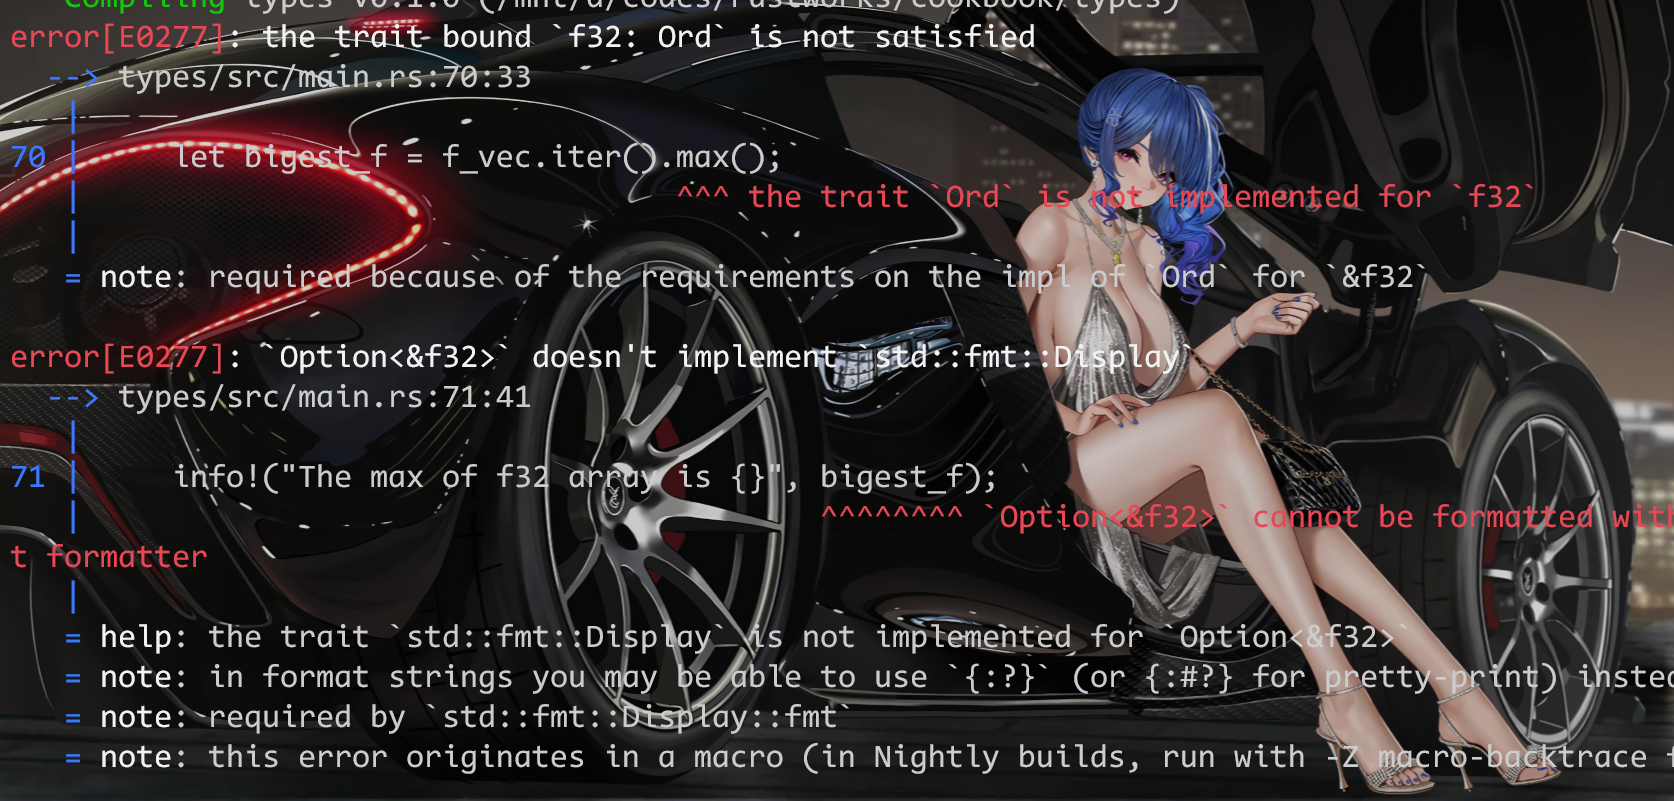
\includegraphics[scale=0.2]{rust_float_cmp_error.png}
  \caption{浮点数的最值错误求解}
  \label{fig:rust_float_cmp_error}
\end{figure}
浮点数的排序只能通过partial\_cmp(比较相等关系)进行变换处理,如下方代码:
\begin{code-block}{rust}
let mut f_vec = vec![1f32, 2.0, 4.0, 0.0, -1.2];
// 升序排列
f_vec.sort_by(|first, second| first.partial_cmp(second).unwrap());
// 获取排序后的最后一位
let max = f_vec.last().unwrap();
// 或者如下进行
// let max = f_vec.as_slice().last().unwrap();
// 降序排列
f_vec.sort_by(|first, second| second.partial_cmp(first).unwrap());
\end{code-block}

作为常用数据类型之一,Rust的数组也存在自己的特点,比如同类型的数组之间可以相互赋值:
\begin{code-block}{rust}
let mut array: [u32; 4] = [1, 23, 4, 5];
let array_copy: [u32; 4] = [5, 6, 7, 8];
array = array_copy;
\end{code-block}
支持数组之间的直接比较,只是数组当中的元素本身就可以进行比较才行:
\begin{code-block}{rust}
let array: [u32; 4] = [1, 23, 4, 5];
let array_copy: [u32; 4] = [5, 6, 7, 8];
info!("{:?}", array < array_copy);
\end{code-block}

Rust当中的函数也可以称之为类型的一种,并且,每个函数都有自己单独的类型,函数的类型
是fn。但是,函数的参数列表会影响fn类型的判断和表达,比如下面的例子:
\begin{code-block}{rust}
fn add_tuple(t: (u32, u32)) -> u32 {
    t.0 + t.1
}

fn add_two((x, y): (u32, u32)) -> u32 {
    x + y
}

fn add_normal(x: u32, y: u32) -> u32 {
    x + y
}

\end{code-block}
实际上,add\_tuple和add\_two这2个函数被fn类型识别成为具有相同签名的类型,因此,
在理论上,我们可以使用同一个变量,接收这2个函数的指针:
\begin{code-block}{rust}
fn main() {
    let mut func = add_tuple;
    func = add_two;
    ...
}
\end{code-block}
但是,上述代码却是错误的:虽然签名相同,但是,类型不同:
\begin{figure}[H]
  \centering
  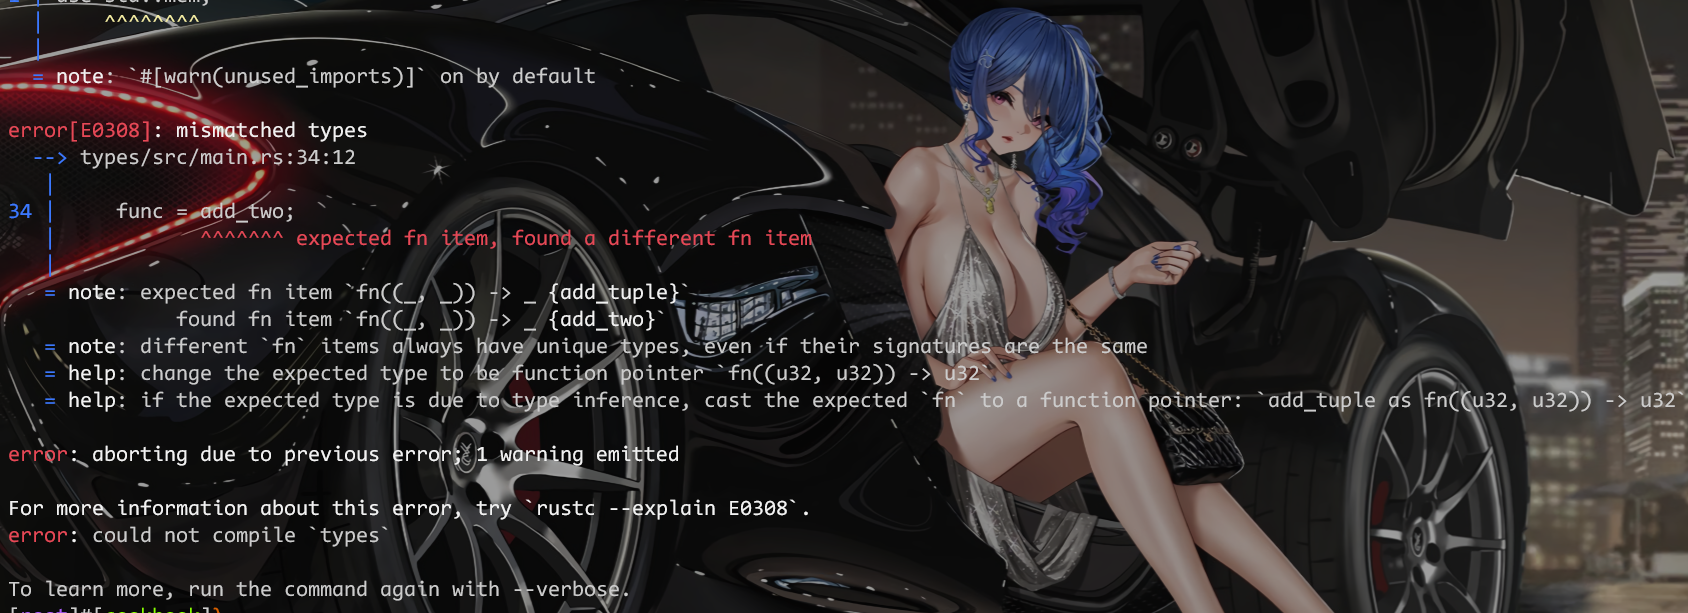
\includegraphics[width=\linewidth]{rust_func_type.png}
  \caption{相同签名的不同函数类型}
  \label{fig:rust_func_type}
\end{figure}
解决方法,则是将其转换成通用的fn类型:
\begin{code-block}{rust}
fn main() {
    // 显示指定func的类型
    let mut func: fn((u32, u32)) -> u32 = add_tuple;
    // 使用as进行类型的转换
    // let mut func = add_tuple as fn((u32, u32)) -> u32;
    func = add_two;
    ...
}
\end{code-block}
但是,需要注意,add\_normal的功能看上去和前面两个函数的功能相同,但是,他们的
函数签名完全不同,因此,不能将其转换成func。

函数是Rust的头等公民,可以在函数/方法当中定义函数,也可以在函数/方法当中定义结构
体,甚至于定义结构体的方法和实现,以及静态变量,常量等:
\begin{code-block}{rust}
fn func_as_first(x: u32, y: u32) -> (u32, u32) {
    struct Point {
        x: u32,
        y: u32,
    };

    impl Point {
        fn area(&self) -> u32 {
            self.x * self.y
        }
        fn cycle(&self) -> u32 {
            self.x + self.y
        }
    };

    let p = Point { x: x, y: y };
    (p.area(), p.cycle())
}
\end{code-block}

常规的函数类型,都会存在返回值,这些返回值要么是特定的类型,要么就是(),即类似
C/C++的返回void。如果需要什么都不返回,则可以使用!,这种函数称之为发散函数,比如
在处理panic时,有时就需要使用发散函数:
\begin{code-block}{rust}
fn diverges() -> ! {
    panic!("This function never returns!");
}
\end{code-block}
Panic操作会直接导致软件栈展开,因此,后续的操作都不会执行,其返回的就是一个!。
发散函数的最大特点,就是可以被转换成任意一个类型,虽然执行的时候最终还是会崩溃,
如下:
\begin{code-block}{rust}
let x : i32 = diverges();
let y : String = diverges();
\end{code-block}
但是,发散函数最大的作用,在于解决编译器的类型检查:
\begin{code-block}{rust}
let p = if x {
    panic!("error");
} else {
    100
};
\end{code-block}
对于let-if而言,if-else的每个分支都必须是相同的数据类型,通过发散函数的任意类型
转换特性即!与任何类型兼容,所以上述代码才能编译通过。

所有的Rust变量,函数都是类型的一种,都可以通过一定的手段和方式,获得类型的具体信息。
常见的方式有两种,一种是使用错误信息进行推断,一种则是使用标准库函数进行获得。

通过构造一个特殊的函数,然后调用该函数,则可以获得相关的类型信息:
\begin{code-block}{rust}
// 接收一个unit参数
fn type_id(_: ()) {}

fn main() {
    let ref i = 5;
    type_id(i);
}
\end{code-block}

而另外的方式,则是使用标准库函数,不过,这个标准库函数在Rust的默认stable分支当中
是不可用的,需要在nightly分支当中进行编译使用,并且,还需要启用一些特性:
\begin{code-block}{rust}
#![feature(core_intrinsics)]
use std;

// 使用泛型参数进行不同类型的数据接收
fn print_type<T>(_arg: &T) {
    println!(
        "The type name of arg is {}",
        std::intrinsics::type_name::<T>()
    );
}

fn main() {
    let ref x = 5;
    print_type(&x);
}
\end{code-block}
编译上述代码时,则需要对编译指令进行部分的调整:
\mintinline[breaklines=true,breakanywhere,breaksymbolleft=,breakanywheresymbolpre=,]{bash}{cargo +nightly build},
然后即可实现对参数类型的打印输出。

在Rust当中,与Python不同,函数/方法并不存在默认参数,但是,结构体当中的字段,却可以
有默认值,只是,这个默认值的实现,必须和Default Trait相结合,如下:
\begin{code-block}{rust}
struct ColoredString {
    input: String,
    fg_color: String,
    bg_color: String,
}

impl Default for ColoredString {
    fn default() -> Self {
        ColoredString {
            input: String::default(),
            fg_color: String::default(),
            bg_color: String::default(),
        }
    }
}

fn main() {
    let color = ColoredString::default();
}
\end{code-block}
从上述代码当中可以看出,实际上,并不是Rust的结构体字段赋予了初始值,而是通过一个
名为default的方法,构造一个我们认为应该具有默认值的结构体。在Rust当中,常用的基本
数据类型都实现了Default Trait,可以直接使用对应的default方法。

\subsection{Trait类型与泛型再论}
关于类型,Trait也是比较重要的一个话题。在之前的示例当中,Trait全部是在具体的类型
上实现的,但是,Trait本身也可以在智能指针(Box)上实现,比如:
\begin{code-block}{rust}
trait Shape {
    fn area(self: Box<Self>) -> f64;
}
struct Circle {
    radius: f64,
}
impl Shape for Circle {
    fn area(self: Box<Self>) -> f64 {
        PI * self.radius * self.radius
    }
}
fn main() {
    let c = Box::new(Circle { radius: 4f64 });
    info!("{}", c.area());
    // 由于trait实现是在智能指针box上,因此,下面的使用是错误的
    // let c = Circle { radius: 4f64 }
    // c.area()
}
\end{code-block}
甚至在Trait上实现Trait,比如下方:
\begin{code-block}{rust}
trait Shape {
    fn area(&self) -> f64;
}
trait Round {
    fn get_radius(&self) -> f64;
}
struct Circle {
    radius: f64,
}
impl Round for Circle {
    fn get_radius(&self) -> f64 {
        self.radius
    }
}
impl Shape for dyn Round {
    fn area(&self) -> f64 {
        let radius = self.get_radius();
        PI * radius * radius
    }
}
\end{code-block}
Shape是一个Trait,Round同样也是一个Trait,Circle实现了Round,Round实现了Shape,
但是,由于Round本身是一个Trait,拥有不确定性,因此,在实现Shape的时候,需要添加
dyn关键字,提示这个Round不是普通的类型,而是一个Trait。上述代码当中,Circle间接
的实现了Shape,但是,Circle的类型无法直接使用Shape的方法,只能通过智能指针的方
式,将Circle转换成Round的类型,再进行使用,如下:
\begin{code-block}{rust}
fn main() {
    let c: Box<dyn Round> = Box::new(Circle { radius: 4f64 });
    info!("{}", c.area());
}
\end{code-block}
如果再把这个例子改得复杂一些,让Circle和Sphere同时实现Round,则我们可以使用Round
指针计算2个不同类型数据的结果:
\begin{code-block}{rust}
trait Shape {
    fn area(&self) -> f64;
}
trait Round {
    fn calc(&self) -> f64;
}
struct Circle {
    radius: f64,
}
impl Round for Circle {
    fn calc(&self) -> f64 {
        PI * self.radius * self.radius
    }
}
struct Sphere {
    radius: f64,
}
impl Round for Sphere {
    fn calc(&self) -> f64 {
        4f64 * PI * self.radius * self.radius
    }
}
impl Shape for dyn Round {
    fn area(&self) -> f64 {
        self.calc()
    }
}
fn main() {
    let circle: Box<dyn Round> = Box::new(Circle { radius: 4f64 });
    info!("The Circle area is {}", circle.area());
    let sphere: Box<dyn Round> = Box::new(Sphere { radius: 4f64 });
    info!("The Sphere area is {}", sphere.area());
}
\end{code-block}

Trait不仅仅用于实现类型,约束类型,还可以用于为其他现有的数据类型添加方法/函数,
比如:
\begin{code-block}{rust}
impl Round for i32 {
    fn calc(&self) -> f64 {
        *self as f64
    }
}
fn main() {
    let i_struct = 4i32;
    i_struct.calc();
}
\end{code-block}
这种类型的函数/方法,则称之为扩展方法/函数。从上述例子当中,我们似乎可以使用Trait
对任意类型进行函数/方法的扩展,但是,这个是存在前提的:
\begin{itemize}
  \item impl和trait的声明/定义在同一个crate当中
  \item 或者,impl的实现需要和类型的声明在同一个crate当中
\end{itemize}
如果不满足上述条件,则容易出现bug和问题,也会违反Rust的规则。

Rust的Trait支持多种特性,自然也支持继承,但是注意,Rust的结构体和enum数据类型并不
存在继承的概念。Trait的继承方式如下:
\begin{code-block}{rust}
trait Base {}
trait Derived : Base {}
\end{code-block}
当一个结构体实现了上述的Derived这个Trait,则必须同样实现Base这个Trait,否则就会
出现语法错误:
\begin{code-block}{rust}
trait Base {}
trait Derived : Base {}
struct T;
impl Derived for T {}
impl Base for T {}
\end{code-block}

Rust的Trait不仅可以包括函数的定义,同样可以直接定义函数:
\begin{code-block}{rust}
trait Page {
    fn set_page(&self) {
        info!("Page Default: 1");
    }
}
trait PerPage {
    fn set_per_page(&self) {
        info!("Per Page Default: 1");
    }
}
struct Paginate {
    page: u32,
}
impl Page for Paginate {}
impl PerPage for Paginate {}
fn main() {
    let page = Paginate { page: 8 };
    page.set_page();
    page.set_per_page();
    page.set_skip_page();
}
\end{code-block}

甚至于,Trait可以直接给结构体提供更多的组合方法:
\begin{code-block}{rust}
trait PaginateMore: Page + PerPage {
    fn set_skip_page(&self) {
        info!("Skip the page");
    }
}
fn main() {
    ...
    page.set_skip_page();
}
\end{code-block}
结构体根本不用自行实现Trait PaginateMore,就可以直接使用该Trait当中的方法。

Trait不仅仅可以用于接口实现,在Rust当中,更重要的则是类型限定,限定某些数据只能
做某些事情。比如下方的代码:
\begin{code-block}{rust}
...
fn static_dispatch<T>(t: &T) where T: Bar {
    ...
}
fn dynamic_dispatch(t : &Bar) {
    ...
}
\end{code-block}
对于实现了Trait Bar的类型来说,上述2个函数,都可以被调用,但是,从语法上,static\_dispatch
由于使用了where,表示参数必须限定在Trait Bar类型,在编译时就能够确定;而dynamic\_dispatch
则从语法上表示,输入的参数必须是Bar的对象,即Trait Object。运行时,Trait Object会根据虚表
指针从虚表当中查出正确的指针,再进行动态调用,属于在运行时确定。

但是并不是每一个Trait都可以当着Trait Object使用,这个和类型大小是否确定有关系。每一个
Trait的隐藏类型参数Self默认限定为?Sized,?Sized trait包括了所有动态大小类型以及所有
可确定大小的类型。Rust当中大部分类型都是默认可确定大小的,即<T:Sized>。当trait对象
在运行期进行动态分发时,也必须确定大小,否则无法分配内存。只有同时满足下列条件的
trait,才可以当作Trait Object使用:
\begin{itemize}
  \item Trait的Self不能被限定为Sized
  \item Trait当中的所有方法都必须是对象安全的
\end{itemize}

而所谓的对象安全,则必须满足如下的条件\underline{\color{red} \textbf{之一}}:
\begin{itemize}
  \item 当Trait的Self被限定为Sized时,方法受Self:Sized约束
  \item Trait的方法签名必须\underline{\color{red} \textbf{同时满足以下3点}}
  \begin{enumerate}
    \item 不包含任何泛型参数(Self)
    \item 第一个参数必须为Self类型或可解引用为Self类型
    \item Self不能出现在除第一个参数之外的其他地方
  \end{enumerate}
  \item Trait当中不能包含关联常量
\end{itemize}

比如下面的代码,就属于标准的对象安全:
\begin{code-block}{rust}
trait Bar {
    fn bax(self, x: u32);
    fn bay(&self);
    fn baz(&mut self);
}
\end{code-block}
Trait Bar不受Sized限制,Trait的方法没有额外的Self类型参数,没有泛型参数,因此是安全的。
相对应的,不安全的Trait如下:
\begin{code-block}{rust}
// 对象不安全
trait Foo {
    fn bad<T>(&self, x:T);
    fn new() -> Self;
}

// 对象安全
trait Foo {
    fn bad<T>(&self, x: T);
    fn new() -> Self
    where
        Self: Sized;
}
\end{code-block}

当然,Sized约束也可以用于Trait定义当中。比如,自行实现一个类似any的Any Trait。
\begin{code-block}{rust}
use std::ops::Fn;
trait CustomAny {
    fn custom_any<F>(&self, f: F) -> bool
    where
        Self: Sized,
        F: Fn(u32) -> bool;
}

impl CustomAny for Vec<u32> {
    fn custom_any<F>(&self, f: F) -> bool
    where
        Self: Sized,
        F: Fn(u32) -> bool,
    {
        for &x in self {
            if f(x) {
                return true;
            }
        }
        false
    }
}

fn main() {
    let v: Vec<u32> = vec![1, 2, 3];
    info!("{}", v.iter().any(|&x| x == 3));
    info!("{}", v.custom_any(|x| x == 3));
}
\end{code-block}

Trait当中不仅可以包含函数和方法,同样可以包含变量和常量,即所谓的关联变量以及关联
常量。关联常量的使用稍微有些特殊,在Trait当中可以定义关联常量,但是,使用的时候,
却是通过Trait的实现对象来使用这些关联常量的:
\begin{code-block}{rust}
trait Colorize {
    // 定义关联常量
    const FG_RED: &'static str = "31";
    const BG_YELLOW: &'static str = "43";
    fn red(self) -> ColoredString;
    fn on_yellow(self) -> ColoredString;
}

impl Colorize for ColoredString {
    fn red(self) -> ColoredString {
        ColoredString {
            // 使用关联常量,如果是Colorize::FG_RED,则会提示错误
            fg_color: String::from(ColoredString::FG_RED),
            ..self
        }
    }
    fn on_yellow(self) -> ColoredString {
        ColoredString {
            bg_color: String::from(ColoredString::BG_YELLOW),
            ..self
        }
    }
}
\end{code-block}

Trait不仅仅可以实现泛型,泛型也不仅限于Trait和<T>,对于函数/方法,也可以使用在
泛型、生命周期以及Trait当中,比如,显式的指定闭包的生命周期:
\begin{code-block}{rust}
// 将函数作为泛型参数
struct Pick<F> {
    data: (u32, u32),
    func: F,
}

impl<F> Pick<F>
where
    // for<>只能用于标记生命周期
    F: for<'f> Fn(&'f (u32, u32)) -> &'f u32,
{
    fn call(&self) -> &u32 {
        (self.func)(&self.data)
    }
}

fn max(data: &(u32, u32)) -> &u32 {
    if data.0 > data.1 {
        return &data.0;
    }
    &data.1
}

fn main() {
    let pick = Pick {
        data: (32, 34),
        func: max,
    };
    info!("{}", pick.call());
}
\end{code-block}

\subsection{常见的设计模式}
建造者模式是Rust当中最常用的设计模式之一,其主旨思想在于将可变和不可变进行分离,
一种基本的示例如下:
\begin{code-block}{rust}
use std::f64::consts;

pub struct Circle {
    radius: f64,
}

pub struct CircleBuilder {
    radius: f64,
}

impl Circle {
    pub fn new() -> CircleBuilder {
        CircleBuilder { radius: 0.0 }
    }

    pub fn area(&self) -> f64 {
        self.radius * self.radius * consts::PI
    }
}

impl CircleBuilder {
    pub fn radius(&mut self, radius: f64) -> &mut CircleBuilder {
        self.radius = radius;
        self
    }
    pub fn build(&self) -> Circle {
        Circle {
            radius: self.radius,
        }
    }
}
\end{code-block}

\subsection{并行与并发再论}
虽然Rust本身的线程/进程管理非常完善,但是,thread::spawn产生的线程没有名称,并且
其栈空间大小默认为2M,如果需要需要针对线程/进程进行粒度更细的操作,比如自定义
线程名称,自定义线程的资源等等,此时,就需要使用thread::Builder进行修改,具体示例
如下:
\begin{code-block}{rust}
let mut v_thread = vec![];
for id in 1..5 {
    let thread_name = format!("child-{}", id);
    let size: usize = 1024;
    // 定义线程的名称,设置线程占用的栈大小为1M(1024)
    let builder = Builder::new().name(thread_name).stack_size(size);
    // builder.spawn返回的是Result<JoinHander, std::io::Error>
    // 需要进行处理,取出真正的线程句柄
    match builder.spawn(move || {
        info!(
            "In the child: {}, and the child name is {}",
            id,
            current().name().unwrap()
        );
    }) {
        Ok(child) => v_thread.push(child),
        Err(error) => error!("Cannot create the thread {} because: {:?}", id, error),
    };
}

// 其他的同普通的线程,
for child in v_thread {
    child.join().unwrap();
}
\end{code-block}

由于线程包含自己的资源空间,因此,存在一个特殊的存储空间——线程本地存储(Thread Local Storage,TLS),
存放在该区域的资源,其他线程无法访问,而是每个线程独占的数据:
\begin{code-block}{rust}
use std::cell::RefCell;
use std::thread;

fn main() {
    // 在线程本地存储定义一个FOO变量,最终的类型是thread::LocalKey
    thread_local!(static FOO: RefCell<u32> = RefCell::new(1));
    // 提供了一个with方法,可以通过给该方法传入闭包
    // 来操作线程本地存储中包含的变量
    FOO.with(|f| {
        info!("The f borrow is {}", *f.borrow());
        *f.borrow_mut() = 2;
    });

    let handler = thread::spawn(move || {
        // 子线程也有一个线程本地存储实例FOO,为主线程的副本
        // 也可以使用thread_local!宏在该子线程中重新创建一个LocalKey实例
        FOO.with(|f| {
            info!("In the handler thread The f borrow is {}", *f.borrow());
            *f.borrow_mut() = 3;
        });
    });

    // 主线程当中FOO实例并没有被子线程修改为3
    // thread local!宏定义单个线程内的一些独享数据
    FOO.with(|f| {
        info!("The f borrow is {}", *f.borrow());
    });

    handler.join().unwrap();
}
\end{code-block}

在同步原语支持方面,Rust也有自己的实现方式,通过使用std::thread当中的park函数提供
阻塞线程的能力,但并不能永久的阻塞线程,存在时间限制;而std::thread::part\_timeout
则可以显式的指定阻塞的超时时间;std::thread::Thread::unpark则可以将阻塞的线程重启;
如果需要让出当前线程的时间片,则需要使用std::thread::yeild\_now,让其他线程进行执行。
简单的阻塞例子如下:
\begin{code-block}{rust}
use std::thread::{self, Builder};
use std::time::Duration;

fn main() {
    let parked_thread = Builder::new()
        .spawn(|| {
            info!("Parking the thread ...");
            // 阻塞当前线程
            thread::park();
            info!("Thread parked");
        })
        .unwrap();
    thread::sleep(Duration::from_secs(5));
    info!("Unparking the thread");
    // 从JoinHandle中得到具体的线程
    parked_thread.thread().unpark();
    // 将该线程重新启动,该线程会继续沿着之前暂停的上下文执行
    parked_thread.join().unwrap();
}
\end{code-block}

除了常见的互斥锁(Mutex)之外,Rust也支持读写锁(RwLock)。读写锁的基本示例如下:
\begin{code-block}{rust}
use std::sync::RwLock;

fn main() {
    let rw_lock = RwLock::new(5);
    // 读写锁的使用必须使用{}进行区分,即便是单独使用读或者写也是一样
    // 通过代码块{},让读写锁自动释放,否则会出现死锁
    {
        let read_1 = rw_lock.read().unwrap();
        let read_2 = rw_lock.read().unwrap();
        info!("The read_1 is {}, and read_2 is {}", read_1, read_2);
    }
    {
        let mut write = rw_lock.write().unwrap();
        *write = 100;
    }
    info!("The data is {:?}", rw_lock);
}
\end{code-block}

而针对于同步的需求,Rust提供了屏障(Barrier)和条件变量(Condition Variable)原语。
屏障,是要求所有的条件全部满足之后,再进行后续操作,即在满足某个条件前,阻塞全部的
线程,通常用于线程同步,如下:
\begin{code-block}{rust}
use std::sync::{Arc, Barrier};
use std::thread;

fn main() {
    let mut vec = vec![];
    let barrier = Arc::new(Barrier::new(5));
    for id in 0..5 {
        let barrier_copy = barrier.clone();
        vec.push(thread::spawn(move || {
            info!("Thread {} Waiting the other threads...", id);
            // wait阻塞了所有的线程,当所有线程的wait之前部分全部执行完成之后
            // wait操作才算执行完成,才会执行每个线程后续的操作
            barrier_copy.wait();
            info!("{} After wait...", id);
        }));
    }

    for handler in vec {
        handler.join().unwrap();
    }
}
\end{code-block}

而条件变量与屏障稍微的区别在于,它不是阻塞所有的线程,而是在满足特定条件前,阻塞
一个得到了互斥锁的线程,如下:
\begin{code-block}{rust}
use std::sync::{Arc, Condvar, Mutex};
use std::thread;
use std::time::Duration;

fn main() {
    // 生成包含互斥锁的条件变量condvar
    let pair = Arc::new(((Mutex::new(false)), Condvar::new()));
    let pair_clone = pair.clone();

    let handler = thread::spawn(move || {
        let &(ref lock, ref cvar) = &*pair_clone;
        // 获得互斥锁
        let mut started = lock.lock().unwrap();
        info!("In the child thread");
        thread::sleep(Duration::from_secs(5));
        *started = true;
        // 通知主线程
        cvar.notify_one();
    });

    let &(ref lock, ref cvar) = &*pair;
    let mut started = lock.lock().unwrap();
    while !*started {
        info!("Waiting for the started singal {} ...", started);
        // 使用条件变量的wait阻塞当前线程,一直到cvar退出
        started = cvar.wait(started).unwrap();
        info!("Started singal finished {} ...", started);
    }
    handler.join().unwrap();
}
\end{code-block}
相比于单纯的互斥锁必须多次出入临界区才能获取到某个状态的信息,条件变量减少了系统
资源的浪费,但是需要注意,每个条件变量每次只能和一个互斥锁(体)一起使用。

除了使用锁、屏障以及条件变量,关于同步的问题,还可以使用原子操作。Rust目前只提供了
4个原子操作类型:AtomicBool、Atomiclsize、AtomicPtr和AtomicUsize。需要注意,虽然原子
操作类型本身可以保证操作的原子性,但是其本身并没有提供跨线程的共享方法,如果需要
使得原子数据类型也可以在线程间共享,则应当使用Arc进行封装,比如下面,使用原子类型
实现一个自旋锁:
\begin{code-block}{rust}
use std::sync::atomic::{AtomicUsize, Ordering};
use std::sync::Arc;

fn main() {
    let spinlock = Arc::new(AtomicUsize::new(1));
    let spinlock_clone = spinlock.clone();
    let handler = thread::spawn(move || {
        // 将原子类型的数据设置为0
        spinlock_clone.store(0, Ordering::SeqCst);
    });

    // 使用spinlock的load方法读取其内部原子类型的值,如果不为0,
    // 则不停地循环测试锁的状态,直到其状态被置为0为止
    // 所谓“自旋”就是指在语义上表示这种不断循环获取锁状态的行为
    while spinlock.load(Ordering::SeqCst) != 0 {}
    handler.join().unwrap();
}
\end{code-block}
代码当中的Ordering表示内存参数顺序,可以通过该参数来控制底层线程执行顺序。默认的,
Rust支持5种内存顺序,归为3大类:
\begin{itemize}
  \item 排序一致性顺序——SeqCst:最简单直观,要求必须先存储,后读取,在多线程环境下,所有的原子写操作都必须在读操作之前完成,强行指定了线程的执行顺序,保证了多线程中所有操作的全局一致性,但是存在性能损耗,其实质类似于餐厅点餐,相当于强制要求所有需要结账的客人,必须等所有点单的客户完成之后才可以结账
  \item 自由顺序——Relaxed:和SeqCst相反,完全不会对线程的顺序进行干涉,线程只进行原子操作,但是,线程之间会存在竞态条件,使用这种内存顺序会比较危险,只有在明确了解当前使用场景且必须使用它的情况下(比如只有读操作),才可使用自由顺序
  \item 获取-释放顺序——Release,Acquire和AcqRel: 是除排序一致性顺序之外的优先选择,默认情况下,不会对全部线程进行统一强制性的执行顺序要求,store表示释放(release),而load表示获取(acquire),通过这2种操作的协作实现线程同步。Release表示使用该顺序的store操作,之前所有的操作对于使用Acquire顺序的load操作都可见;反之,使用使用Aquire顺序的load操作,对于使用Release的store操作都是可见的;AcqRel表示读时使用Acquire顺序的load操作,写时使用Release顺序的store操作。获取释放顺序虽然不像排序一致性顺序那样对全局线程统一排序,但是它让每个线程都能接固定的顺序执行。
\end{itemize}

\subsection{常见错误处理方法}
由于很多代码都是第三方的,而Rust本身也在不断的发展,有可能出现版本不兼容或者特性
不兼容的情况,此时,则需要进行相关的修改。比如下面的一种错误:
\begin{figure}[H]
  \centering
  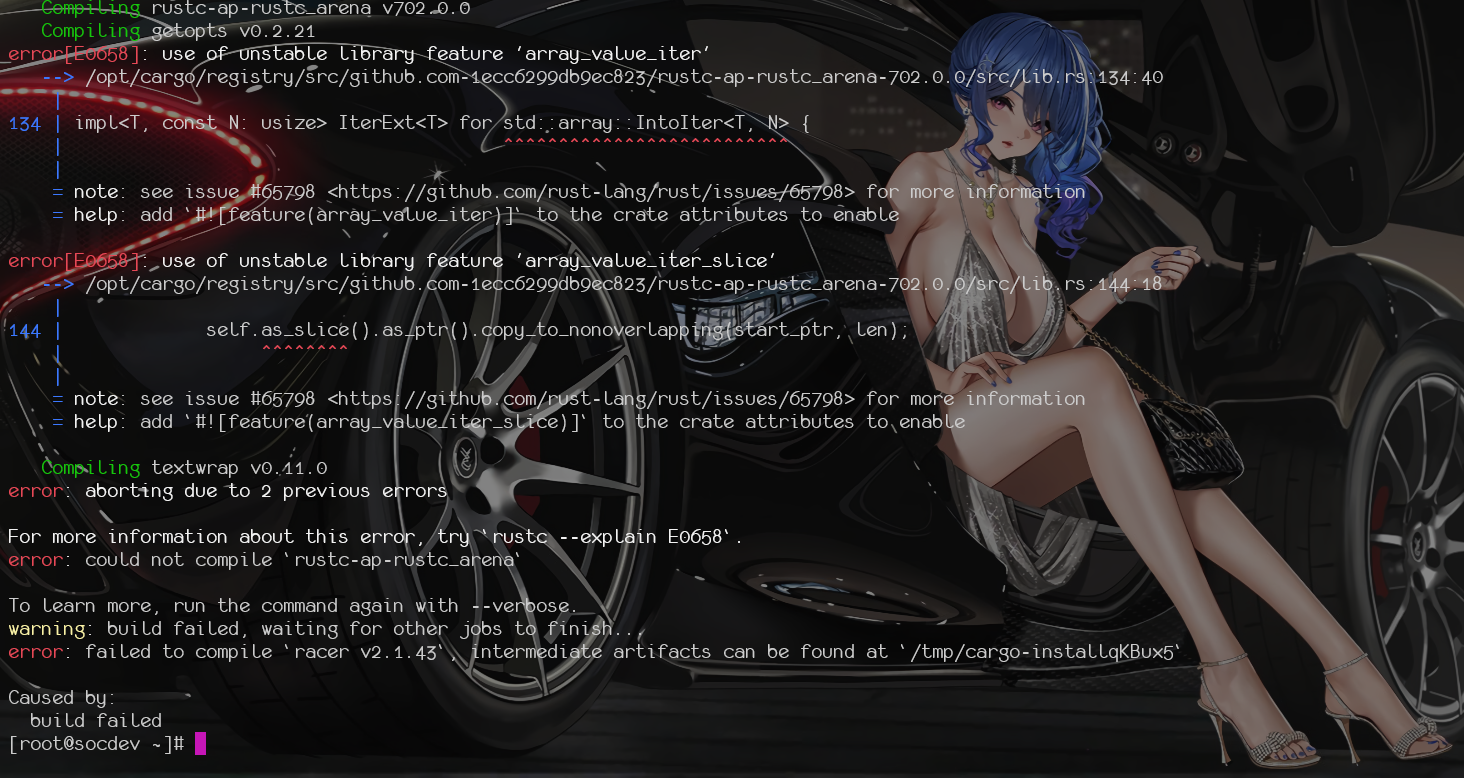
\includegraphics[width=\linewidth]{rust_feature_error.png}
  \caption{缺少特性支持编译失败}
  \label{fig:rust_feature_error}
\end{figure}
遇到这种错误,则需要直接修改对应的类库的源代码。以上述错误为例,编译的help表示
\mintinline[breaklines=true,breakanywhere,breaksymbolleft=,breakanywheresymbolpre=,]{bash}{add `#![feature(array_value_iter_slice)]` to the crate attributes to enable},
则我们应当在对应的crate的lib.rs的头部当中,添加内容如下:
\begin{figure}[H]
  \centering
  
\includegraphics[width=\linewidth]{rust_feature_add.png}
  \caption{增加特性支持}
  \label{fig:rust_feature_add}
\end{figure}


